%%%%%%%%%%%%%%%%%%%%%%%%%%%%% Define Article %%%%%%%%%%%%%%%%%%%%%%%%%%%%%%%%%%
\documentclass[12pt]{article}
%%%%%%%%%%%%%%%%%%%%%%%%%%%%%%%%%%%%%%%%%%%%%%%%%%%%%%%%%%%%%%%%%%%%%%%%%%%%%%%

%%%%%%%%%%%%%%%%%%%%%%%%%%%%% Using Packages %%%%%%%%%%%%%%%%%%%%%%%%%%%%%%%%%%
\usepackage{geometry}
\usepackage{graphicx}
\usepackage{amssymb}
\usepackage{amsfonts}
\usepackage{amsmath}
\usepackage{yhmath}
\usepackage{amsthm}
\usepackage{mathrsfs}
\usepackage{enumitem}
\usepackage{empheq}
\usepackage{mdframed}
\usepackage{booktabs}
\usepackage{lipsum}
\usepackage{graphicx}
\usepackage{hyperref}
\usepackage{color}
\usepackage{psfrag}
\usepackage{pgfplots}
\usepackage{bm}
%%%%%%%%%%%%%%%%%%%%%%%%%%%%%%%%%%%%%%%%%%%%%%%%%%%%%%%%%%%%%%%%%%%%%%%%%%%%%%%

% Other Settings
\graphicspath{ {./figures/} }

\makeatletter
\@beginparpenalty=1000000
\makeatother

%%%%%%%%%%%%%%%%%%%%%%%%%% Page Setting %%%%%%%%%%%%%%%%%%%%%%%%%%%%%%%%%%%%%%%
\geometry{a4paper}

%%%%%%%%%%%%%%%%%%%%%%%%%% Define some useful colors %%%%%%%%%%%%%%%%%%%%%%%%%%
\definecolor{ocre}{RGB}{243,102,25}
\definecolor{mygray}{RGB}{243,243,244}
\definecolor{deepGreen}{RGB}{26,111,0}
\definecolor{shallowGreen}{RGB}{235,255,255}
\definecolor{deepBlue}{RGB}{61,124,222}
\definecolor{shallowBlue}{RGB}{235,249,255}
%%%%%%%%%%%%%%%%%%%%%%%%%%%%%%%%%%%%%%%%%%%%%%%%%%%%%%%%%%%%%%%%%%%%%%%%%%%%%%%

%%%%%%%%%%%%%%%%%%%%%%%%%% Define an orangebox command %%%%%%%%%%%%%%%%%%%%%%%%
\newcommand\orangebox[1]{\fcolorbox{ocre}{mygray}{\hspace{1em}#1\hspace{1em}}}
%%%%%%%%%%%%%%%%%%%%%%%%%%%%%%%%%%%%%%%%%%%%%%%%%%%%%%%%%%%%%%%%%%%%%%%%%%%%%%%

%%%%%%%%%%%%%%%%%%%%%%%%%%%% English Environments %%%%%%%%%%%%%%%%%%%%%%%%%%%%%
\newtheoremstyle{mytheoremstyle}{3pt}{3pt}{\normalfont}{0cm}{\rmfamily\bfseries}{}{1em}{{\color{black}\thmname{#1}~\thmnumber{#2}}\thmnote{\,--\,#3}}
\newtheoremstyle{myproblemstyle}{3pt}{3pt}{\normalfont}{0cm}{\rmfamily\bfseries}{}{1em}{{\color{black}\thmname{#1}~\thmnumber{#2}}\thmnote{\,--\,#3}}
\theoremstyle{mytheoremstyle}
\newmdtheoremenv[linewidth=1pt,backgroundcolor=shallowGreen,linecolor=deepGreen,leftmargin=0pt,innerleftmargin=20pt,innerrightmargin=20pt,]{theorem}{Theorem}[section]
\newmdtheoremenv[linewidth=1pt,backgroundcolor=mygray,linecolor=deepGreen,leftmargin=0pt,innerleftmargin=20pt,innerrightmargin=20pt,]{corollary}{Corollary}[section]
\newmdtheoremenv[linewidth=1pt,backgroundcolor=mygray,linecolor=ocre,leftmargin=0pt,innerleftmargin=20pt,innerrightmargin=20pt,]{lemma}{Lemma}[section]
\newmdtheoremenv[linewidth=1pt,backgroundcolor=mygray,linecolor=ocre,leftmargin=0pt,innerleftmargin=20pt,innerrightmargin=20pt,]{proposition}{Proposition}[section]
\theoremstyle{mytheoremstyle}
\newmdtheoremenv[linewidth=1pt,backgroundcolor=shallowBlue,linecolor=deepBlue,leftmargin=0pt,innerleftmargin=20pt,innerrightmargin=20pt,]{definition}{Definition}[section]
\theoremstyle{myproblemstyle}
\newmdtheoremenv[linecolor=black,leftmargin=0pt,innerleftmargin=10pt,innerrightmargin=10pt,]{problem}{Problem}[section]


%\newtheorem{theorem}{Theorem}[subsection]
%\newtheorem{lemma}[theorem]{Lemma}
\newtheorem{claim}[theorem]{Claim}
%\newtheorem{proposition}[theorem]{Proposition}
% \newtheorem{corollary}[theorem]{Corollary}
\newtheorem{fact}[theorem]{Fact}
\newtheorem{notation}[theorem]{Notation}
\newtheorem{observation}[theorem]{Observation}
\newtheorem{conjecture}[theorem]{Conjecture}
%%%%%%%%%%%%%%%%%%%%%%%%%%%%%%%%%%%%%%%%%%%%%%%%%%%%%%%%%%%%%%%%%%%%%%%%%%%%%%%

%%%%%%%%%%%%%%%%%%%%%%%%%%%%%%% Plotting Settings %%%%%%%%%%%%%%%%%%%%%%%%%%%%%
\usepgfplotslibrary{colorbrewer}
\pgfplotsset{width=8cm,compat=1.9}
%%%%%%%%%%%%%%%%%%%%%%%%%%%%%%%%%%%%%%%%%%%%%%%%%%%%%%%%%%%%%%%%%%%%%%%%%%%%%%%

%%%%%%%%%%%%%%%%%%%%%%%%%%%%%%% Custom Shortcuts %%%%%%%%%%%%%%%%%%%%%%%%%%%%%%

% Norm and Abs
\DeclarePairedDelimiter{\abs}{\lvert}{\rvert}
\DeclarePairedDelimiter{\norm}{\lVert}{\rVert}

% "blackboard-fonted" letters for the reals, naturals etc.
\newcommand{\R}{\mathbb R}
\newcommand{\N}{\mathbb N}
\newcommand{\Z}{\mathbb Z}
\newcommand{\F}{\mathbb F}
\newcommand{\Q}{\mathbb Q}
\newcommand{\C}{\mathbb C}
\newcommand{\T}{\mathbb T}

% blackboard letters
\newcommand{\bbA}{\mathbb{A}}
\newcommand{\bbB}{\mathbb{B}}
\newcommand{\bbC}{\mathbb{C}}
\newcommand{\bbD}{\mathbb{D}}
\newcommand{\bbE}{\mathbb{E}}
\newcommand{\bbF}{\mathbb{F}}
\newcommand{\bbG}{\mathbb{G}}
\newcommand{\bbH}{\mathbb{H}}
\newcommand{\bbI}{\mathbb{I}}
\newcommand{\bbJ}{\mathbb{J}}
\newcommand{\bbK}{\mathbb{K}}
\newcommand{\bbL}{\mathbb{L}}
\newcommand{\bbM}{\mathbb{M}}
\newcommand{\bbN}{\mathbb{N}}
\newcommand{\bbO}{\mathbb{O}}
\newcommand{\bbP}{\mathbb{P}}
\newcommand{\bbQ}{\mathbb{Q}}
\newcommand{\bbR}{\mathbb{R}}
\newcommand{\bbS}{\mathbb{S}}
\newcommand{\bbT}{\mathbb{T}}
\newcommand{\bbU}{\mathbb{U}}
\newcommand{\bbV}{\mathbb{V}}
\newcommand{\bbW}{\mathbb{W}}
\newcommand{\bbX}{\mathbb{X}}
\newcommand{\bbY}{\mathbb{Y}}
\newcommand{\bbZ}{\mathbb{Z}}

% calligraphic letters
\newcommand{\cA}{\mathcal{A}}
\newcommand{\cB}{\mathcal{B}}
\newcommand{\cC}{\mathcal{C}}
\newcommand{\cD}{\mathcal{D}}
\newcommand{\cE}{\mathcal{E}}
\newcommand{\cF}{\mathcal{F}}
\newcommand{\cG}{\mathcal{G}}
\newcommand{\cH}{\mathcal{H}}
\newcommand{\cI}{\mathcal{I}}
\newcommand{\cJ}{\mathcal{J}}
\newcommand{\cK}{\mathcal{K}}
\newcommand{\cL}{\mathcal{L}}
\newcommand{\cM}{\mathcal{M}}
\newcommand{\cN}{\mathcal{N}}
\newcommand{\cO}{\mathcal{O}}
\newcommand{\cP}{\mathcal{P}} \newcommand{\cQ}{\mathcal{Q}} \newcommand{\cR}{\mathcal{R}}
\newcommand{\cS}{\mathcal{S}}
\newcommand{\cT}{\mathcal{T}}
\newcommand{\cU}{\mathcal{U}}
\newcommand{\cV}{\mathcal{V}}
\newcommand{\cW}{\mathcal{W}}
\newcommand{\cX}{\mathcal{X}}
\newcommand{\cY}{\mathcal{Y}}
\newcommand{\cZ}{\mathcal{Z}}

% fraktur letters
\newcommand{\fA}{\mathfrak{A}}
\newcommand{\fB}{\mathfrak{B}}
\newcommand{\fC}{\mathfrak{C}}
\newcommand{\fD}{\mathfrak{D}}
\newcommand{\fE}{\mathfrak{E}}
\newcommand{\fF}{\mathfrak{F}}
\newcommand{\fG}{\mathfrak{G}}
\newcommand{\fH}{\mathfrak{H}}
\newcommand{\fI}{\mathfrak{I}}
\newcommand{\fJ}{\mathfrak{J}}
\newcommand{\fK}{\mathfrak{K}}
\newcommand{\fL}{\mathfrak{L}}
\newcommand{\fM}{\mathfrak{M}}
\newcommand{\fN}{\mathfrak{N}}
\newcommand{\fO}{\mathfrak{O}}
\newcommand{\fP}{\mathfrak{P}}
\newcommand{\fQ}{\mathfrak{Q}}
\newcommand{\fR}{\mathfrak{R}}
\newcommand{\fS}{\mathfrak{S}}
\newcommand{\fT}{\mathfrak{T}}
\newcommand{\fU}{\mathfrak{U}}
\newcommand{\fV}{\mathfrak{V}}
\newcommand{\fW}{\mathfrak{W}}
\newcommand{\fX}{\mathfrak{X}}
\newcommand{\fY}{\mathfrak{Y}}
\newcommand{\fZ}{\mathfrak{Z}}

% hats
\newcommand{\hatA}{\widehat{A}}
\newcommand{\hatB}{\widehat{B}}
\newcommand{\hatC}{\widehat{C}}
\newcommand{\hatD}{\widehat{D}}
\newcommand{\hatE}{\widehat{E}}
\newcommand{\hatF}{\widehat{F}}
\newcommand{\hatG}{\widehat{G}}
\newcommand{\hatH}{\widehat{H}}
\newcommand{\hatI}{\widehat{I}}
\newcommand{\hatJ}{\widehat{J}}
\newcommand{\hatK}{\widehat{K}}
\newcommand{\hatL}{\widehat{L}}
\newcommand{\hatM}{\widehat{M}}
\newcommand{\hatN}{\widehat{N}}
\newcommand{\hatO}{\widehat{O}}
\newcommand{\hatP}{\widehat{P}}
\newcommand{\hatQ}{\widehat{Q}}
\newcommand{\hatR}{\widehat{R}}
\newcommand{\hatS}{\widehat{S}}
\newcommand{\hatT}{\widehat{T}}
\newcommand{\hatU}{\widehat{U}}
\newcommand{\hatV}{\widehat{V}}
\newcommand{\hatW}{\widehat{W}}
\newcommand{\hatX}{\widehat{X}}
\newcommand{\hatY}{\widehat{Y}}
\newcommand{\hatZ}{\widehat{Z}}

% hats
\newcommand{\hata}{\widehat{a}}
\newcommand{\hatb}{\widehat{b}}
\newcommand{\hatc}{\widehat{c}}
\newcommand{\hatd}{\widehat{d}}
\newcommand{\hate}{\widehat{e}}
\newcommand{\hatf}{\widehat{f}}
\newcommand{\hatg}{\widehat{g}}
\newcommand{\hath}{\widehat{h}}
\newcommand{\hati}{\widehat{i}}
\newcommand{\hatj}{\widehat{j}}
\newcommand{\hatk}{\widehat{k}}
\newcommand{\hatl}{\widehat{l}}
\newcommand{\hatm}{\widehat{m}}
\newcommand{\hatn}{\widehat{n}}
\newcommand{\hato}{\widehat{o}}
\newcommand{\hatp}{\widehat{p}}
\newcommand{\hatq}{\widehat{q}}
\newcommand{\hatr}{\widehat{r}}
\newcommand{\hats}{\widehat{s}}
\newcommand{\hatt}{\widehat{t}}
\newcommand{\hatu}{\widehat{u}}
\newcommand{\hatv}{\widehat{v}}
\newcommand{\hatw}{\widehat{w}}
\newcommand{\hatx}{\widehat{x}}
\newcommand{\haty}{\widehat{y}}
\newcommand{\hatz}{\widehat{z}}


%%%%%%%%%%%%%%%%%%%%%%%%%%%%%%% Title & Author %%%%%%%%%%%%%%%%%%%%%%%%%%%%%%%%
\title{Master's Project}
\author{Joel Sleeba}
%%%%%%%%%%%%%%%%%%%%%%%%%%%%%%%%%%%%%%%%%%%%%%%%%%%%%%%%%%%%%%%%%%%%%%%%%%%%%%%

\begin{document}
    \maketitle
    % TeX root = main.tex
\section{Preface}
I plan to write and detail everything(almost) I study and learn for my Master's project into these latex files. I assume it will be much easier to track whatever I have learned and to have a good overview of the topic with this note taking. Also since I am doing it on \LaTeX\ I am sure it will save me from the last minute rush to type everything out and make the report of the project. I will start with Fourier series and will introduce new concepts when they are required as we go along. So, let us start


Joel Sleeba\\
\today

\newpage

\section{Preliminaries}

  \subsection{Measure theory}

  \begin{definition}[$\sigma$-algebra]
    \label{def:sigma_algrebra}
    A collection $\Sigma$ of subsets of a set $X$ is called a $\sigma$-algebra if it satisfy the following properties
    \begin{enumerate}
      \item $X\in \Sigma$
      \item If $E \in \Sigma$, then $E^c \in \Sigma$.
    \item If $E_1, E_2, \dots$ are elements of $\Sigma$, then $\bigcup_{i=1}^\infty E_i \in \Sigma$.
    \end{enumerate}
  \end{definition}

    % TeX root = main.tex
\newpage
\section{Fourier Series in $L^1(\T)$}

  \subsection{Definition and basic properties}

    We'll begin by reviewing the definition of $L^p$ space since we'll be mostly working on functions from these space.
  \begin{definition}[$L^p$ function]
    \label{def:Lp_function}
    A real valued function $f$ defined on a lebesgue measure space $S$ is called an $L^p$ function on $S$ or a $p$-integrable function on $S$ if 
    \begin{displaymath}
       \left( \int_{S} |f(x)|^p \right)^{1/p} < \infty
    \end{displaymath}
    For such a function the integral above is called the $p$-norm of the function $f$ and often denoted by $\|f\|_{L^p(S)}$ or $\|f\|_p$ if the space is known.
\end{definition}  
  Although we've defined general $L^p$ spaces, we'll mostly be concerned about $L^1$ and $L^2$ functions in $\R$ and $\T = [0, 1)$ .
  \\

  Now let's define what a periodic function is.
  \begin{definition}[Periodic function]
    \label{def:periodic_function}
    A function $f:\R \to \R$ is called periodic with period $p$(or $p$-periodic) if $f(x+p) = f(x)$ for all $x \in \R$

  \end{definition}
  Although we're definining real valued periodic functions the definition holds well for any function $f$ from the reals to a space where equality is defined.
  Also note that if we know the value of a $p$ periodic function $f$ in a closed-open (or open-close or closed) interval of length $p$ say $[x, x+p)$, then using the definition of periodic function we can get the function value at the whole of $\R$(we leave it for the reader to verify). That is, we can identify any $p$ periodic function $f$ on $\R$ with the restriction of $f$ onto an interval of length $p$. We can also identify $f$ with the values in a unit circle in $\C$.
  Specifically we'll be working with $1$-periodic functions identified by their restrictions in $\T$.
\\

  \begin{definition}[Continuous functions in $\T$]
    \label{def:continuous_functions_on_T}
    Continuous functions on $\T$, are precisely those functions which are continuous in $\R$ with period $1$. We'll denote the collection of continuous functions in $\T$ with $C(\T)$.
  \end{definition}

  Now let's prove an important result of periodic functions.
  \begin{lemma}
    \label{lem:integral_of_periodic_function}
    If $f:\R \to \R$ is of period $1$ and $\int_{0}^{1} f(x) dx$ exists, then for any real number $a$, 
    \begin{displaymath}
      \int_{a}^{a+1}f(x) dx = \int_{0}^{1} f(x) dx
    \end{displaymath} 
  \end{lemma}
  \begin{proof}
    Let $a = n +b$, where $0\le b <1$ and $n$ is an integer. Then since $f$ has period 1,
    \begin{displaymath}
      \int_{a}^{a+1}f(x) dx = \int_{n+b}^{n+b+1}f(x)dx = \int_{b}^{b+1}f(x+n)dx = \int_{b}^{b+1}f(x)dx
    \end{displaymath}
    and, 
    \begin{align*}
      \int_{b}^{b+1}f(x)dx &= \int_{b}^{1}f(x)dx + \int_{1}^{b+1}f(x)dx \\
                      &= \int_{b}^{1}f(x)dx + \int_{0}^{b}f(x+1)dx \\
                      &= \int_{b}^{1}f(x)dx + \int_{0}^{b}f(x)dx \\
                      &= \int_{0}^{1}f(x)dx
    \end{align*}

    Hence the result.
    
  \end{proof}

  Now we'll define fourier coefficients of a periodic function $f \in L^1(\T)$
  \begin{definition}[Fourier coefficient]
    \label{def:fourier_coefficient}
    Let $f \in L^1(\T)$, i.e $\int_{\T} f < \infty$. Then for each integer $n$ we define the $n^{th}$ fourier coefficient, $\hatf(n)$ as 
    \begin{displaymath}
      \hatf(n) = \int_0^1 f(x)e^{-2\pi inx} dx \end{displaymath}
  \end{definition}
  $\hatf(n)$ is finite and well defined for each $n$ since $f \in L^1(\T)$, since
  \begin{displaymath}
    |\hatf(n)| \le \int_0^1 |f(x)e^{-2\pi inx}| dx \le \int_0^1 |f(x)||e^{-2\pi inx}| dx = \int_0^1|f(x)| dx < \infty
  \end{displaymath}
  
  Once we have the fourier coefficients of a function at hand we can combine them together to make a series called the fourier series. We'll be investigating the conditions at which this series converges to our initial function $f$.

  Also note that the map which takes $f$ to $\hatf$ is linear since if $f, g \in L^1(\T)$, then $$\widehat{f+g}(n) = \int_0^1 (f+g)(x) e^{-2 \pi inx} \ dx = \int_0^1f(x)e^{-2\pi inx} \ dx + \int_0^1g(x)e^{-2\pi inx} \ dx = \hatf(n) + \hatg(n)$$ and for some $\lambda \in \R$, $$\widehat{\lambda f}(n) \ dx = \int_0^1 \lambda f(x) e^{-2\pi inx} \ dx = \lambda \int_0^1 f(x) e^{-2 \pi inx} \ dx = \lambda\hatf(n)$$

  \begin{definition}[Fourier series]
    \label{def:fourier_series}
    Given a function $f \in L^1(\T)$, the fourier series of the function $f$ is defined as 
    \begin{displaymath}
      \sum_{n\in \Z} \hatf(n)e^{2\pi inx}
    \end{displaymath}
    where $\hatf(n)$ is the $n^{th}$ fourier coefficient as defined in \ref{def:fourier_coefficient} 
  \end{definition}

  \begin{proposition}[Properties of Fourier coefficinets]
    \label{prop:properties_of_fourier_coefficients}
    Suppose that $f\in L^1(\T)$.
    \begin{enumerate}[label=(\alph*)]
      \item If $a$ is a real number and $g(x) = f(x+a)$ for all $x$, then $\hatg(n) = \hatf(n)e^{2\pi ina}$ for all $n \in \Z$.
      \item if $b$ is an integer and $h(x) = f(x)e^{2\pi i bx}$ for all $x$, then $\hath(n) = \hatf(n-b)$ for all $n\in \Z$.
      \item if $j(x) = f(-x)$ for all $x$, then $\hatj(n) = \hatf(-n)$
    \end{enumerate}
  \end{proposition}
  \begin{proof}
     Given $f(x) \in L^1(\T)$ and $n^{th}$ Fourier coefficient of $f$,  
    \[\hatf(n) = \int_{0}^{1}f(x)e^{-2 \pi inx}.\]
    \begin{enumerate}
      \item[(a)] Then, the $n^{th}$ Fourier coefficient of $g(x) = f(x+a)$ is
        \begin{align*}
          \hatg(n) &= \int_{0}^{1}g(x)e^{-2\pi inx} dx \\
                &= \int_{0}^{1}f(x+a)e^{-2\pi inx} dx \\
                &= \int_{0}^{1}f(x)e^{-2\pi in(x-a)} dx \\
                &= e^{2\pi ina} \int_0^1 f(x)e^{-2\pi inx} dx \\
                &= e^{2\pi ina} \hatf(n)
        \end{align*}

      \item[(b)] If $h(x) = f(x)e^{2\pi ibx}$, then
        \begin{displaymath}
          \hath(n) = \int_0^1 f(x)e^{-2 \pi i (n-b)x} dx = \hatf(n-b)
        \end{displaymath}
      \item[(c)] $j(x) = f(-x)$, then
        \begin{align*}
          \hatj(n)  &= \int_0^1 f(-x)e^{-2\pi inx} dx \\
                    &= -\int_0^{-1} f(y) e^{2\pi iny}dy & \text{by } y=-x\\
                    &= \int_{-1}^0 f(y)e^{2\pi iny}dy \\
                    &= \int_0^1 f(y)e^{2\pi iny}dy & \text{by lemma }\ref{lem:integral_of_periodic_function}\\
                    &= \hatf(-n)
        \end{align*}
        
        
    \end{enumerate}
  \end{proof}


  \subsection{Convolution}
  Now we'll define another important operation with function called the convolution of two functions.
  \begin{definition}
    Let $f, g \in L^1(\T)$, then the convolution of $f$ and $g$ is defined as 
    \begin{displaymath}
      f*g(x) = \int_0^1 f(y)g(x-y)dy
    \end{displaymath}
  \end{definition}

  Convolution can be thought of as taking the moving average of a function with another function. Refer figure \ref{fig:convolution}.
  \begin{figure}
    \centering
    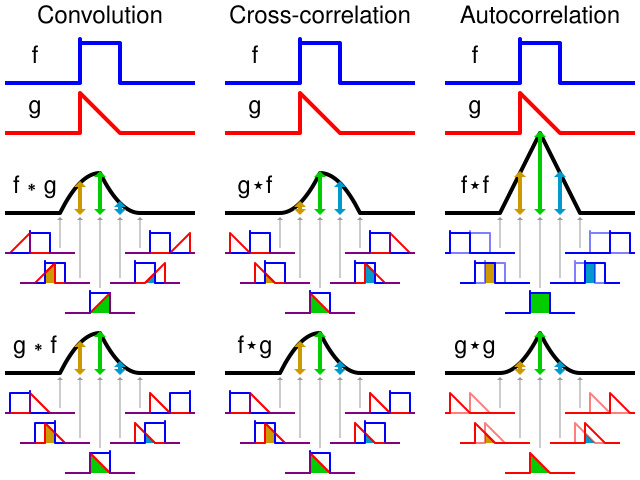
\includegraphics[width=0.6\textwidth]{convolution}
    \caption{convolution}
    \label{fig:convolution}
  \end{figure}

  \begin{proposition}[Properties of convolution]
    \label{prop:properties_of_convolution}
    Let $f, g \in L^1(\T)$, then 
    \begin{enumerate}[label=(\alph*)]
      \item $f*g = g*f$
      \item $f*(g+h) = f*g +f*h$
      \item $(cf)*g = c(f*g)$
      \item $f*(g*h) = (f*g)*h$
    \end{enumerate}
  \end{proposition}
  \begin{proof}
    We'll just prove the commutativity and will leave the rest for the reader to verify. (Hint: Use properties of integration)

    Put $v = x-y$, we get $dv = -dy$ and 
    \begin{align*}
      f*g(x)  &= \int_{0}^{1}f(y)g(x-y) dy \\
              &= -\int_{x}^{x-1} f(x - v)g(v) dy\\
              &= \int_{x-1}^{x} g(v)f(x-v) dy \\
              &= \int_{0}^{1}g(v)f(x-v)dy  &\text{by lemma } \ref{lem:integral_of_periodic_function}\\
              &=g*f(x)
    \end{align*} 
  \end{proof}
  

  We'll prove another important result that the convolution of two $L^1(\T)$ functions is again in $L^1(\T)$.
  \begin{theorem}
    \label{thm:convolution_is_in_L1}
  Let $f, g \in L^1(\T)$. Then $h = f*g \in L^1(\T)$, and $\hath(n) = \hatf(n)\hatg(n)$.
  \end{theorem}
  % \begin{proof}
  %   Consider the function $h: \T^2 \to \T$ defined as $h(x, y) = f(x)$. Then
  %   \begin{align*}
  %     h^{-1}(a, 1) &= \{(x, y)\in \T^2, h(x,y) > a \} \\
  %                 &= \{(x, y)\in \T^2, f(x) > a \} \\
  %                 &= f^{-1}(a, 1)\times \T
  %   \end{align*}
  %   Similarly, define $k(x, y): \T^2 \to \T$ as $k(x, y) = g(y)$. Then we'll get $k^{-1}(b, 1) = \T \times g^{-1}(b, 1)$ like above. 
  %   Since $f, g$ are measurable functions in $\T$, $f^{-1}(a, 1), g^{-1}(b, 1)$ are measurable sets in $\T$ and hence $h, k$ are measurable functions in $\T^2$.
  %   
  %   Then $F(x, y): \T^2 \to \T$ defined as $F(x, y) = f(x)g(y)$ is a measurable function, since $F^{-1}((a, b)\times (c, d)) = f^{-1}(a, b) \times g^{-1}(c, d)$ which is again open for any open set $(a, b)\times (c, d)$ in $\T^2$
  %
  %   Again $T: \T^2 \to \T$ defined as $T(x, y) = (x,x-y)$ is measurable being linear. Hence $H: \T^2 \to \T$ defined as $H(x, y) = F \circ T (x, y) = f(x)g(x-y)$ is measurable being the composition of measurable functions. 
  %   
  % \end{proof}

  \begin{proof}
    \begin{align*}
  \int_{0}^{1} |h(x)| dx &= \int_{0}^{1} \left| \int_{0}^{1} f(y)g(x-y)\  dy \right| dx \\
                         &\le \int_{0}^{1} \int_{0}^{1} |f(y)g(x-y)| \ dy \ dx \\
                         &= \int_{0}^{1} \int_{0}^{1} |f(y)g(x-y)| \ dx \ dy & \text{by Tonelli's theorem}\\
                         &= \int_{0}^{1} \left( \int_{0}^{1} |g(x-y)| dx \right) |f(y)|dy \\
                         &=\norm{f}_1 \norm{g}_1
    \end{align*}

    Note that we're using Tonelli's theorem here to interchange the limits of integration since the space is a finite measure space. This proves that $h = f*g \in L^1(\T)$.

    To prove the next part,
    \begin{align*}
      \hath(n) &= \int_0^1 \left( \int_0^1 f(y)g(x-y)dy \right) e^{-2\pi in x} dx \\
               &= \int_0^1 f(y) \left( \int_0^1 g(x-y) e^{-2\pi in x}dx \right) dy & \text{by Tonelli's theorem}\\  
               &= \int_0^1 f(y) \hatg(n)e^{-2\pi inx} dy & \text{by proposition } \ref{prop:properties_of_fourier_coefficients} \text{(a)}\\
               &= \hatf(n)\hatg(n)
    \end{align*}
  \end{proof}
 

  \subsection{Partial sums of Fourier series}
  Given a function $f$ in the $\T$, we are interested in the convergence of fourier series of $f$. We'll discuss about the convergence of the symmetric partial sum of the Fourier series.

  \begin{definition}[Symmetric partial sum of a Fourier series]
    \label{def:symmetric_partial_sum_of_fourier_series}
    Given a function $f \in \L^1(\T)$ with its fourier series, $\sum_{-\infty}^\infty \hatf(n)e^{2\pi in x}$, we define the $n^{th}$ symmetric parial sum of the fourier series as
    \begin{displaymath}
      S_N(x) = \sum_{n=-N}^N \hatf(n)e^{2\pi inx}
    \end{displaymath}
  \end{definition}
  But it may happen that the summetric partial sum of the Fourier seies may not converge. To deal with this we'll define another partial sum called the Ces\'aro partial sum.

  \begin{definition}[Ces\'aro partial sum of Fourier series]
    \label{def:cesaro_partial_sum_of_fourier_series}
    Given a function $f \in \L^1(\T)$ with its Fourier series, $\sum_{-\infty}^\infty \hatf(n)e^{2\pi in x}$, we define the $n^{th}$ Ces\'aro parial sum of its Fourier series as
    \begin{displaymath}
      \sigma_N(x) = \frac{1}{N}\sum_{n=0}^{N-1} S_n(x)
    \end{displaymath}
    where $S_n(x)$ is the symmetric partial sum of the Fourier series as defined in \ref{def:symmetric_partial_sum_of_fourier_series}
  \end{definition}
  For an example, $\{-1^{n}\}$ is a sequence whose symmetric partial sums do not converge but the Ces\'aro partial sums converge to $\frac{1}{2}$. Also if the symmetric partial sums of a series converge, then the Ces\'aro partial sums will also converge to the same limit. \textcolor{red}{(Prove it!)}

  Now we'll show that the Ces\'aro partial sum can be rewritten to another form which will help our proofs down the road.
  \begin{lemma}
    \label{lem:property_of_cesaro_partial_sum}
    If $\sigma_N(x)$ is the $N^{th}$ Ces\'aro partial sum of the Fourier series of a function $f\in L^1(\T)$, then
    \begin{displaymath}
      \sigma_N(x) = \sum_{n=-N}^N \left(1-\frac{\abs{n}}{N} \right) \hatf(n) e^{2\pi inx}
    \end{displaymath}
  \end{lemma}
  \begin{proof}
    We'll prove the result for a general series so that it'll help us also in Fourier series.

    Let $S_N = \sum_{n=-N}^{N}a_n$ be the $N^{th}$ partial sum of the series $\sum_{-\infty}^{\infty}a_n$. Then by the definition of Ces\'aro partial sum, 
    \begin{align*}
      \sigma_N  &= \frac{1}{N} \sum_{n=0}^{N-1}S_n \\
                &= \frac{1}{N} \sum_{n=0}^{N-1}\sum_{k=-n}^{n}a_k \\
                &= \frac{1}{N} \sum_{k=-N+1}^{N-1} a_k \sum_{n=|k|}^{N-1} 1 \\
                &= \frac{1}{N} \sum_{k=-N+1}^{N-1} \left(N - |k|\right) a_k \\
                &=  \sum_{k=-N+1}^{N-1} \left(1 - \frac{|k|}{N}\right) a_k \\
                &=  \sum_{k=-N}^{N} \left(1 - \frac{|k|}{N}\right) a_k \\ 
    \end{align*}
    Now speficially if we take $a_k = \hatf(k)e^{2\pi ikx}$, we get the required result. 
  \end{proof}

  \subsection{Summability Kernels}
  Now we'll define a family of functions called the sumambility kernels, which we will use heavily in our proofs and simplify it.
  \begin{definition}[Summability kernel]
    \label{def:summability_kernel}
    A sequence of functions $K_N \in L^1(\T)$ is called a summability kernel or an approximation identity if 
    \begin{enumerate}[label=(\alph*)]
      \item $\int_{0}^{1}K_N(x)dx = 1$
      \item $\int_{0}^{1}\abs{K_N(x)}dx \le C$ for some constant $C>0$
      \item $\lim_{N\to\infty} \int_{\delta}^{1-\delta}\abs{K_N(x)}dx= 0$
    \end{enumerate}
  \end{definition}
 

  Now we'll define one of the important summability kernels.
  \begin{definition}[Fej\'er kernel]
    \label{def:fejer_kernel}
    Fej\'er kernel is defined as a collection of functions  $\Delta_N$ where for each $N \in \N$, $\Delta_N : \R \to \R$ is defined as 
    \begin{displaymath}
      \Delta_N(x) = \sum_{n=-N}^{N}\left( 1 - \frac{\abs{n}}{N}\right)e^{2\pi inx}
    \end{displaymath}
  \end{definition}
  Notice that each $\Delta_N$ is a $1-$periodic function.

  We'll prove that Fej\'er kernel as defined in \ref{def:fejer_kernel} satify the properties in \ref{def:summability_kernel}. But before that we'll explore some properties of Fej\'er kernel so that it'll aid us in our proof.
  \begin{proposition}[Properties of Fej\'er kernel]
    \label{prop:properties_of_fejer_kernel}
    If $\Delta_N(x)$ is defined as in \ref{def:fejer_kernel}, then the following hold true
    \begin{enumerate}[label=(\alph*)]
      \item
        $$\Delta_N(x) = 1 + 2 \sum_{n=1}^{N} ( 1-\frac{n}{N} )\cos{2\pi nx}$$ 
      \item
        $$\int_0^1 \Delta_N(x) dx = 1$$
      \item 
        $$\Delta_N(x) = \Delta_N(1-x)$$
    
\item For $0\le \delta \le \frac{1}{2}$,
        $$\int_\delta^{\frac{1}{2}} \Delta_N(x) dx = \int_{\frac{1}{2}}^{1 - \delta} \Delta_N(x) dx$$
        and therefore,
        $$\int_0^{\frac{1}{2}} \Delta_N(x) dx = \int_{\frac{1}{2}}^{1} \Delta_N(x) dx = \frac{1}{2}$$
      
      \item
        \begin{displaymath}
          \Delta_N(x) = 
            \begin{cases}
              \frac{1}{N}\left( \frac{\sin(\pi Nx)}{\sin(\pi x)} \right)^2, &\text{ if } x\notin \Z \\
              N, &\text{ if } x \in \Z\
            \end{cases}
        \end{displaymath}
      \item
        If $0\le x \le \frac{1}{2}$, then $$\Delta_N(x) \le \min\left(N, \frac{1}{4Nx^2}\right)$$
      \item 
        If $0<\delta \le \frac{1}{2}$, then 
        $$\int_\delta^{\frac{1}{2}}\Delta_N(x) < \frac{1}{4N\delta}$$
      \item 
        \begin{displaymath}
          (\Delta_N*f)(x) = \sigma_N(x) 
        \end{displaymath}
        where $\sigma_n(x)$ is the $n^{th}$ Ces\'aro partial sum of the Fourier series of $f$ as defined in $\ref{def:cesaro_partial_sum_of_fourier_series}$
    \end{enumerate}
  \end{proposition}

  \begin{proof}
    \begin{enumerate}[label=(\alph*)]
      \item
        This follows straight from De Moivre's formula that $e^{ix} = \cos(x) + i\sin(x)$ and $e^{ix} + e^{-ix}  = 2\cos(x)$.

      \item 
        By previous result,
          $$\Delta_N(x) = 1 + 2\sum_{n=1}^N \left(1-\frac{|n|}{N}\right)\cos(2\pi nx)$$
        Therefore, 
        \begin{align*}
          \int_0^1\Delta_N(x) \ dx &= \int_0^1 1\ dx + 2\sum_{n=1}^N \left(1 - \frac{|n|}{N}\right)\int_0^1cos(2\pi nx) \ dx \\
                &= 1 + 0 \\ 
        \end{align*}

      \item
        This follows from the fact that $\cos(2\pi n(1-x))  = \cos(2\pi n - 2\pi nx) = \cos(2\pi nx)$ in the last result.
      \item
        From \ref{prop:properties_of_fejer_kernel}, we know that $\Delta_N(x) = \Delta_N(1-x)$. Therefore by change of variables,
        \begin{displaymath}
          \int_\delta^{\frac{1}{2}}\Delta_N(x) dx = \int_\delta^{\frac{1}{2}}\Delta_N(1-x)dx = -\int_{1-\delta}^{\frac{1}{2}} \Delta_N(y)dy = \int_{\frac{1}{2}}^{1 - \delta}\Delta_N(y) dy
        \end{displaymath}
        Also from previous result, we know
        $$\int_0^{\frac{1}{2}}\Delta_N(x) dx + \int_{\frac{1}{2}}^1\Delta_N(x) dx = \int_0^1\Delta_N(x) dx = 1$$
        Hence $$\int_0^{\frac{1}{2}} \Delta_N(x) dx = \int_{\frac{1}{2}}^1 \Delta_N(x) dx = \frac{1}{2}$$

      \item
        If $x\in \N$ then $e^{2\pi inx} = 1$ for all $n$ and then,
        \begin{displaymath}
          \sum_{n=0}^{N-1}e^{2\pi inx} = \sum_{n=0}^{N-1} 1 = N
        \end{displaymath}
        Hence the last case is solved. But if $x\notin \N$ then from the finite sum of geometric series,
        \begin{align*}
          \sum_{n=0}^{N-1}e^{2\pi inx} &= \frac{e^{2\pi iNx} - 1}{e^{2\pi ix} - 1} \\
                  & = \frac{e^{\pi iNx}}{e^{\pi ix}} \times \frac{e^{\pi iNx} - e^{-\pi iNx}}{e^{\pi ix} - e^{-\pi ix}} \\
                  & = e^{\pi i(N-1)x}\frac{\sin(\pi Nx)}{\sin(\pi x)}
        \end{align*}
        Since $\abs{e^{ix}} = 1$ for all $x\in \R$, we'll get
        \begin{displaymath}
          \left|\sum_{n=0}^{N-1}e^{2 \pi inx}\right|^2 = \frac{\sin^2(\pi Nx)}{\sin^2(\pi x)}  
        \end{displaymath}

        But we also know that,
        \begin{align*}
         \left|\sum_{n=0}^{N-1}e^{2 \pi inx}\right|^2 &= \left(\sum_{n=0}^{N-1}e^{2 \pi inx}\right)  \left(\sum_{n=0}^{N-1}\overline{e^{2 \pi inx}}\right) \\
            &= \sum_{m=0}^{N-1} \sum_{n=0}^{N-1} e^{2\pi i(m-n)x} \\
            &= \sum_{k = -(N-1)}^{N-1} e^{2\pi ikx} \sum_{\substack{0\le m \le N-1 \\ 0 \le n \le N-1 \\ m-n = k}}1 \\
            &= \sum_{k = -(N-1)}^{N-1} e^{2\pi ikx} (N - |k|) \\
            &= N\Delta_N(x)
        \end{align*}

        Which implies that 
        \begin{displaymath}
          \Delta_N(x) = \frac{1}{N}\frac{\sin^2(\pi Nx)}{\sin^2{\pi x}}
        \end{displaymath}
        Hence the proposition.
     
      \item 
        We'll first see that $\sin(\pi x) \ge 2x$ whenever $0\le x\le \frac{1}{2}$. 
        But this is because the $h(x) := \sin(\pi x) - 2x = 0$ only for $x=0$ and $x=2$ and the derivative of $h$, $h'(x) := \pi \cos(\pi x) - 2 = 0$, only for a unique real number $r\in [0, \frac{1}{2}]$.Now since $f$ is smooth, $f$ cannot have more roots in $[0, \frac{1}{2}]$. Hence $\sin(\pi x) \ge 2x$ for all $x \in [0, \frac{1}{2}]$

        Now we'll get to the main proof. Assume $0 < \delta \le \frac{1}{2}$. Then by previous result, when $0<x \le \frac{1}{2}$,
       \begin{align*}
         \Delta_N(x) &= \frac{1}{N}\left(\frac{\sin(\pi Nx)}{\sin(\pi x)}\right)^2 \\
                &\le \frac{1}{N\sin^2(\pi x)} \\
                &\le \frac{1}{4Nx^2} &\text{since } \sin(\pi x) \ge 2x \\
       \end{align*}

        We also know that $$\Delta_N(x) = 1+ 2 \sum_{n=1}^{N} \left(1-\frac{n}{N}\right)\cos(2\pi nx)$$
        But this shows that $\Delta_N(x)$ is maximum when $\cos(2\pi nx)$ is maximum, i.e at $x = 0, 1$. At both cases $\cos(2\pi nx) = 1$.
        Also $$1 + 2\sum_{n=1}^N \left(1-\frac{n}{N}\right) = 1 + 2N - \frac{2}{N}\sum_{n=1}^N n = 1+2N - \frac{2}{N}\frac{N(N+1)}{2} = N$$
        Therefore, $\Delta_N(x) \le N$ for all $0\le x \le 1$
        Hence combining this with the result above, we get that while $0\le x\le \frac{1}{2}$
        $$\Delta_N(x) \le \min{\left(N, \frac{1}{4Nx^2}\right)}$$

      
     \item
       From last result we know that when $0< \delta \le \frac{1}{2}$, $$\Delta_N(x) \le \frac{1}{4Nx^2}$$
       Then,
        \begin{displaymath}
          \int_\delta^\frac{1}{2} \Delta_N(x) dx \le \int_\delta^\frac{1}{2} \frac{1}{4Nx^2} dx \le \int_\delta^\infty \frac{1}{4Nx^2} dx = \frac{1}{4N\delta}
        \end{displaymath}

    \item
      \begin{align*}
        (\Delta_N*f)(x) &= \int_0^1 \Delta_N(y)f(x-y) \ dy \\
              &= \int_0^1 \sum_{n=-N}^{N} \left(1-\frac{\abs{n}}{N}\right)e^{2\pi iny} f(x-y) \ dy \\
              &= \sum_{n=-N}^N  \left(1-\frac{\abs{n}}{N}\right) \int_0^1 f(x-y) e^{2\pi iny} \ dy \\
              &= \sum_{n=-N}^N  \left(1-\frac{\abs{n}}{N}\right) e^{2 \pi inx}  \int_0^1 f(x-y) e^{-2\pi in \left( x-y \right) } \ dy \\
              &= \sum_{n=-N}^N  \left(1-\frac{\abs{n}}{N}\right) e^{2 \pi inx} \int_x^{x-1} -f(v) e^{-2\pi in v} \ dv \\
              &= \sum_{n=-N}^N  \left(1-\frac{\abs{n}}{N}\right) e^{2 \pi inx} \int_{x-1}^x f(v) e^{-2\pi in v} \ dv \\
              &= \sum_{n=-N}^N  \left(1-\frac{\abs{n}}{N}\right) e^{2 \pi inx} \int_0^{1} f(v) e^{-2\pi in v} \ dv & \text{by lemma } \ref{lem:integral_of_periodic_function}\\
              &= \sum_{n=-N}^N  \left(1-\frac{\abs{n}}{N}\right) e^{2 \pi inx} \hatf(n) \\
              &= \sigma_N(x)
      \end{align*}
    \end{enumerate}
\end{proof}
  

  \begin{proposition}
    \label{prop:fejer_kernel_is_summability_kernel}
    Fej\'er kernel as defined in \ref{def:fejer_kernel} is a summability kernel as in definition \ref{def:summability_kernel}
  \end{proposition}
  \begin{proof}
    To prove that Fej\'er kernel is a summability kernel, we'll verify the three properties given in \ref{def:summability_kernel}.
    \begin{enumerate}
      \item
        We proved that $\int_0^1 \Delta_N(x) = 1$ at proposition \ref{prop:properties_of_fejer_kernel}
      \item
        From proposition \ref{prop:properties_of_fejer_kernel}, we know that
        \begin{displaymath}
          \Delta_N(x) = 
          \begin{cases}
            \frac{1}{N} \left(\frac{\sin(\pi Nx)}{\sin(\pi x)}\right)^2, &\text{ if } x \notin \Z \\
            N, &\text{ if } x \in \Z \\
          \end{cases}
        \end{displaymath}
        Since $N \in \N$, this implies $\Delta_N(x) \ge 0$. Therefore,
        \begin{displaymath}
          \int_0^1 \left|\Delta_N(x)\right| dx = \int_0^1 \Delta(x) dx = 1
        \end{displaymath}
        This proves the $2^{nd}$ condition for the summability kernel.
        
      \item
        To prove that 
        \begin{displaymath}
          \lim_{N \to \infty}\int_\delta^{1-\delta} \left|\Delta_N(x) \right| dx = 0
        \end{displaymath}

        we note that from proposition \ref{prop:properties_of_fejer_kernel} if $0< \delta \le \frac{1}{2}$, $$ \int_\delta^{\frac{1}{2}}\Delta_N(x) dx \le \frac{1}{4N\delta}$$
        and 
        $$\int_\frac{1}{2}^{1-\delta} \Delta_N(x) =  \int_\delta^\frac{1}{2} \Delta_N(x)$$

        Hence,
        \begin{displaymath}
          \int_\delta^{1-\delta} \Delta_N(x) = \int_\delta^\frac{1}{2} \Delta_N(x) + \int_\frac{1}{2}^{1-\delta} \Delta_N(x) = 2 \int_\delta^\frac{1}{2} \Delta_N(x) \le \frac{1}{2N\delta}
        \end{displaymath}
       
        Therefore, for $0 < \delta \le \frac{1}{2}$, we have 
        \begin{displaymath}
          \lim_{N \to \infty} \int_\delta^{1-\delta} \left|\Delta_N(x)\right| = \lim_{N \to \infty} \int_\delta^{1-\delta} \Delta_N(x) = 0
        \end{displaymath}

        If $\frac{1}{2} < \delta < 1$ then by change of variable $y = 1 - x$
        \begin{displaymath}
          \lim_{N\to \infty} \int_\delta^{1-\delta} \Delta_N(x) = \lim_{N \to \infty} - \int_{1-\delta}^{\delta} \Delta_n(y) = 0
        \end{displaymath}
        And therefore for all $0 < \delta < 1$ 
        \begin{displaymath}
          \lim_{N \to \infty} \int_\delta^{1-\delta} \left|\Delta_N(x)\right| =  0
        \end{displaymath}


      Which completes the proof that  Feje\'r kernel is a summability kernel.
    \end{enumerate}
  \end{proof}


  \subsection{Convergence of Fourier Series} % (fold)
  \label{ssub:Convergence of Fourier Series}

  Now with the help of summability kernels and convolution we'll prove an important theorem which will serve as a backbone for the discussion of convergence forward.
  \begin{theorem}[Convergence to convolution of summability kernels]
    \label{thm:L1_convergence_of_summability_kernel}
    If $f\in L^1(\T)$ and $K_N$ is a summability kernel then $f*K_N$ converges to $f$ in $L^1$ norm. That is
    \begin{displaymath}
      \lim_{N\to \infty} \int_{0}^{1}\abs{f(x) - (f*K_N)(x))} = 0
    \end{displaymath}
\end{theorem}
  \begin{proof}
    \begin{displaymath}
      f*K_N(x) = \int_0^1 f(x-y)K_N(y)dy
    \end{displaymath}
    Since $\int_0^1 K_N(y)dy = 1$, by the $2^{nd}$ property of summability kernel,
    \begin{displaymath}
      f(x) - f*K_N(x) = \int_0^1\left(f(x)-f(x-y)\right)K_N(y)dx
    \end{displaymath}
    Now then, 
    \begin{align*}
      \int_0^1 |f(x) - K_N(x)| dx &= \int_0^1 \left| \int_0^1 (f(x) - f(x-y))K_N(y)dy \ \right| \ dx \\
                &\le \int_0^1 \int_0^1 \left| f(x) - f(x-y) K_N(y) \right| dy \ dx \\
                &= \int_0^1 |K_N(y)| \int_0^1 |f(x) - f(x-y)| dx \ dy & \text{by Tonelli's theorem} \\
                &= \int_{-\delta}^{1-\delta} & \text{by lemma } \ref{lem:integral_of_periodic_function}\\
                &= \int_{-\delta}^{\delta} + \int_{\delta}^{1-\delta} = I_1 + I_2\\
    \end{align*}
    We'll show that for a given $\epsilon$ we can find an $N$ such that for all $n>N, \ I_1+I_2 < \epsilon$

    Since $f \in L^1(\T)$ we can find $\delta >0$ such that $\int_0^1| f(x+\delta) - f(x) | dx = \epsilon / 2C$, where $C$ is the constant in the second conditon of summability kernel. The proof can be found in any measure theory textbook.
    
    Then, 
    \begin{displaymath}
      |I_1| \le \frac{\epsilon}{2C} \int_{-\delta}^{\delta}|K_N(y)|dy \le \frac{\epsilon}{2C} \int_0^1 |K_N(y)| dy \le \frac{\epsilon}{2}
    \end{displaymath}  
    
    For $I_2$, we see that 
    \begin{displaymath}
      \int_0^1 |f(x) - f(x-y)|dx \le \int_0^1 |f(x)| dx + \int_0^1 |f(x-y)| dx = 2\norm{f}_1
    \end{displaymath}
  Then,
  \begin{displaymath}
    |I_2| \le 2\norm{f}_1 \int_{\delta}^{1-\delta} |K_N(y)|dy
  \end{displaymath}
But by the $3^{rd}$ property of the summability kernel, we know that the integral in the above converges to zero. Therefore there exists an $N$ such that for an $n>N, |I_2|< \epsilon/2$, which completes our proof.
  \end{proof}

  \begin{corollary}{Convergence of Ces\'aro sum of functions in $L^1(\T)$}
    If $f\in L^(\T)$ then $\sigma_N(x)$, the Ces\'aro sum of the Fourier series of $f$ converge to $f(x)$ in $L^1$ norm. That is, 
    \begin{displaymath}
      \lim_{N\to \infty} \int_0^1 \left|f(x) - \sigma_N(x)\right| = 0
    \end{displaymath}
  \end{corollary}
  \begin{proof}
    Since we know that Fej\'er kernel, $\Delta_N(x)$ is a summability kernel by proposition \ref{prop:fejer_kernel_is_summability_kernel} and that $(\Delta_N*f)(x) = \sigma_N(x)$ by prop \ref{prop:properties_of_fejer_kernel}, the result follows from theorem \ref{thm:L1_convergence_of_summability_kernel}.
  \end{proof}

  \begin{theorem}[Fej\'er's Theorem]
    \label{fejer_theorem}
    Let $f \in L^1(\T)$ and $f(a^-) = \lim_{x \to a^-} f(x)$ and $f(a^+) = \lim_{x \to a^+} f(x)$ exist and are finite, then
    $$\lim_{ N\to \infty} \sigma_N(x) = \frac{f(x^-) + f(x^+)}{2}$$
  \end{theorem}

  \begin{proof}
    Let $\epsilon$ be given. Since we assumed $f(x^+)$ and $f(x^-)$ exist and are finite, we can take $\delta < \frac{1}{2}$ small enough such that $|f(x-u) - f(x^-)| < \epsilon$ for $0\le u \le \delta$ and $|f(x+u) - f(x^+)| < \epsilon$ for $1-\delta \le u \le 1$.
    $$ \sigma_N(x) = \int_0^1 f(x-u)\Delta_N(u) du = \int_{0}^\delta + \int_\delta^{1-\delta} + \int_{1-\delta}^1 = I_1 + I_2 + I_3$$
    Then, 
    $$I_1 = \int_0^\delta (f(x-u) - f(x^-))\Delta_N(u)du + \int_0^\delta f(x^-)\Delta_N(u)du = T_1 + T_1^{'}$$
    where by the property of summability kernels as in \ref{def:summability_kernel}, and by our choice of $\delta$, we have
    $$|T_1| \le \int_0^\delta |f(x-u) - f(x^-)|\Delta_N(u)du < \epsilon \int_0^\delta \Delta_N(x) \le \epsilon$$
    Therefore $T_1$ converge to $0$ as $N \to \infty$.

    Again, from the proposition \ref{prop:properties_of_fejer_kernel}, we get
    $$\frac{1}{2} \ge \int_0^\delta \Delta_N(x) dx = \int_0^{\frac{1}{2}} \Delta_N(x) dx - \int_\delta^{\frac{1}{2}} \Delta_N(x) dx \ge \frac{1}{2} - \frac{1}{4N\delta}$$
    which then implies that, 
    $$\frac{f(x^-)}{2} \ \ge \ T_1^{'} = f(x^-)\int_0^\delta \Delta_N(x) dx \ \ge \ \frac{f(x^-)}{2} - \frac{f(x^-)}{4N\delta}  $$
    Therefore, 
    $$ 0\ge T_1^{'} - \frac{f(x^-)}{2} \ge -\frac{f(x^-)}{4N\delta} $$
    and hence, 
    $$\left| T_1^{'} - \frac{f(x^-)}{2}\right| \le \left|\frac{f(x^-)}{4N\delta}\right| $$
    which implies that $I_1 = T_1 + T_1^{'}$ converge to $\frac{f(x^-)}{2}$ as $N \to \infty$.

    Now by proposition \ref{prop:properties_of_fejer_kernel} we know that if $0 < x \le \frac{1}{2}$, then $$\Delta_N(x) \le \frac{1}{4Nx^2}$$ which implies that 
    $$ |I_2| \le \frac{1}{4N\delta^2}\int_\delta^{1-\delta}f(x-u) du \le \frac{1}{4N\delta^2}\int_0^1|f(u)|du = \frac{\|f\|_1}{4N\delta^2}$$
    Therefore $I_2$ converge to $0$ as $N \to \infty$

    Now we'll prove that $I_3$ converge to $\frac{f(x^+)}{2}$. For this we'll split $I_3$ into $T_3$ and $T_3^{'}$ like we did with $I_1$. 
    $$I_3 = \int_{1-\delta}^1 (f(x-u) - f(x^+))\Delta_N(u) du + f(x^+)\int_{1-\delta}^{1}\Delta_N(u) du = T_3 + T_3^{'}$$
    Then, 
    $$|T_3| \le \int_{1-\delta}^1 |((f(x-u) - f(x^+))|\Delta_N(u)du < \epsilon \int_{1-\delta}^1 \Delta_N(x) dx \le \epsilon$$
    Therefore $T_3$ converge to $0$ as $N \to \infty$.
    Also
      $$\int_{1-\delta}^1 \Delta_N(x) dx = -\int_{\delta}^0 \Delta_N(x) dx = \int_0^\delta \Delta_N(x) dx$$
      Therefore by the same inequality we used for $T_1^{'}$ in \ref{prop:properties_of_fejer_kernel}, we'll get
      $$ \left| T_3^{'} - \frac{f(x^+)}{2} \right| \le \left|\frac{f(x^+)}{4N\delta} \right|$$
      which implies that $I_3 = T_3 + T_3^{'}$ converge to $\frac{f(x^+)}{2}$ as $N \to \infty$

    Therefore since $\sigma_N(x) = I_1 + I_2 + I_3$, by the algebra of limits, 
    $$ \lim_{N \to \infty} \sigma_N(x) = \frac{f(x^-) + f(x^+)}{2}$$
  \end{proof}

 \begin{theorem}[Hardy Tauberian Theorem]
   Let $\sum_{n=1}^\infty a_n$ is Ces\'aro summable to $a$, then if there exist a constant $C$ such that $$|a_n| \le \frac{C}{n}$$ for all $n$, then the series $\sum_{n=1}^\infty a_n$ converge to $a$
 \end{theorem}

    % TeX root = main.tex
\chapter{Fourier Series in $L^p(\T)$}
Before we go into the general $L^p$, we'll first recall some importatnt results from functional analysis which are essential for the discussion of further topics.

Recall that in \autoref{def:Lp_function}, we've discussed what is an $L^p$ function for a general space $S$. Here the space is $\T$ and $L^p(\T)$ are precisely the set of all $L^p$ functions in $\T$.

\begin{theorem}[Holder's Inequality]
   \label{thm:Holder_inequality}
  Let $1 \le  p \le \infty$ and $q$ such that $1/p + 1/q = 1$ (for convention we will assume that the tuples $(1, \infty)$, and $(\infty, 1)$, satify the above relation) then for lebesgue measure space $S$ and functions $f \in L^p(S)$, and $g \in L^q(S)$
  $$ \left| \int_S f(x)g(x) dx \right| \le \|f\|_p \|g\|_q$$
  where $$\|f\|_p = \left(\int_s |f(x)|^p \right)^{\frac{1}{p}}$$ as in \autoref{def:Lp_function}.
\end{theorem}

\begin{theorem}[Minkowski's Inequality]
  \label{thm:Minkowski_inequality}
  Let $1 \le p \le \infty$ then for a lebesgue measure space $S$ and a fucntion $f \in L^p(S)$, then 
  $$\|f+g\|_p \le \|f\|_p + \|g\|_p$$
\end{theorem}

The proofs of the above two theorems can be found in any measure theory textbook and since it is a common proof, we'll ommit it from detailing it here.

\section{Fourier Series in $L^2(\T)$}
Before we proceed with the fourier coefficients and fourier series for $L^2(\T)$ functions we first prove some important results.
\begin{proposition}
  \label{prop:L2_functions_are_continuous_in_L2_norm}
  If $f \in L^2(\T)$, then
  \begin{displaymath}
   \lim_{\delta \to 0} \int_0^1 |f(x+\delta) - f(x)|^2 dx = 0
  \end{displaymath}
\end{proposition}
\begin{proof}
  From measure theory we know that continuous functions are dense in $L^2(\T)$. Then given any $\epsilon$ there exists a function $g\in C(\T)$ such that $\|f-g\|_2 < \epsilon$. Then,
  $$ f(x+\delta) - f(x) = (f(x+\delta) - g(x+\delta)) - (f(x) - g(x)) + ( g(x+\delta) - g(x))$$
  Now by triangle inequality, (i.e minkowski's inequality for $p = 2$), 
  $$ \|f(x+\delta) - f(x)\|_2 = \|f(x+\delta) - g(x+\delta)\|_2 - \|f(x) - g(x)\|_2 + \|g(x+\delta) - g(x)\|_2$$
  Now since $g$ is continuous on $\T$ it is uniformly continuous (since it is continuous on $\R$, it'll be continuous on $[0,1]$, a compact set) and therefore $\delta$ can be taken such that $\|g(x+\delta) - g(x) \|_2 < \epsilon$. Hence the theorem.
\end{proof}

\begin{proposition}
  \label{prop:convolution_of_L2_functions}
  If $f, g \in L^2(\T)$, then their convolution, $f*g$ is continuous and moreover $\|f*g\|_{\infty} \le \|f\|_2 \|g\|_2$
\end{proposition}
\begin{proof}
  $$(f*g)(x+\delta) - (f*g)(x) = \int_0^1 f(u)(g(x+\delta - u) - g(x-u)) du $$
  Therefore by Cauchy Shwarz inequality, 
  \begin{align*}
    |f*g(x+\delta) - f*g(x)| &= \left| \int_0^1 f(u) (g(x + \delta -u)- g(x-u)) du \right| \\
          &\le \|f\|_2 \left( \int_0^1|g(x+\delta - u) - g(x-u)|^2 du \right)^{1/2} \\
  \end{align*}
  which converge to zero as $\delta \to 0$ by \autoref{prop:L2_functions_are_continuous_in_L2_norm}. Therefore $f*g$ is continuous in $\T$.
  Also, 
  \begin{align*}
    |f*g(x)| &= \left| \int_0^1 f(u)g(x-u) du \right| \\
            &\le \left(\int_0^1 |f(u)|^2 du \right)^{1/2} \left(\int_0^1 |g(u)|^2 du \right)^{1/2} \\
            &= \|f\|_2 \|g\|_2
  \end{align*}
  Hence the theorem.
\end{proof}

 Now that we've proved some important results, we'll define the fourier coeffients $\hatf(n)$ the same way we defined them for $\L^1(\T)$ in \autoref{def:fourier_coefficient} as 
$$\hat{f}(n) = \int_0^1 f(x)e^{-2\pi inx} dx$$

Note that $\hatf(n)$ is a finite quantity since $|e^{ix}| = 1$ and,
$$ |\hatf(n)| = \left| \int_0^1 f(x)e^{-2\pi inx} dx \right| \le \|f\|_2\left(\int_0^1 |e^{-2\pi inx}|^2 dx\right)^{1/2} = \|f\|_2 $$

Hence we define the fourier series the same way as in \autoref{def:fourier_series}. Then we'll investigate if the Fourier series of $L^2(\T)$ functions are Ces\'aro summable to $f$. In fact this is true.

\begin{theorem}[Fourier series of $L^2(\T)$ functions are Ces\'aro summable]
  If $f\in L^2(\T)$, and $\sigma_N(x)$ is the $N^{th}$ Ces\'aro partial sum of the Fourier series of $f$, then
  $$ \lim_{N \to \infty} \int_0^1 |f(x) - \sigma_N(x)|^2 \ dx = 0$$
\end{theorem}

\begin{proof}
  From \autoref{prop:properties_of_fejer_kernel} we know that
  \begin{displaymath}
    \sigma_N(x) = \int_0^1 \Delta_N(u)f(x-u) \ du 
  \end{displaymath}
  Hence,
  $$ f(x) - \sigma_N(x) = \int_0^1 (f(x) - f(x-u))\Delta_N(u) \ du $$ 
  By Holder's inequality in \autoref{thm:Holder_inequality} applied to $(f(x) - f(x-u))\sqrt{\Delta_N(u)}$ and $\sqrt{\Delta_N(u)}$ 
  \begin{align*}
    |f(x) - \sigma_N(x)| &= \left| \int_0^1 (f(x) - f(x-u))\Delta_N(u) \right| \ du \\
          &\le \left( \int_0^1 |f(x) - f(x-u)|^{2} \Delta_N(u) \ du \right)^{1/2} \left( \int_0^1 \Delta_N(u) \ du \right)^{1/2} \\
  \end{align*}
  Since by \autoref{prop:properties_of_fejer_kernel}, $\int_0^1 \Delta_N(x) dx = 1$ and by Tonelli's theorem, 
  \begin{align*}
    \int_0^1 |f(x) - \sigma_N(x)|^2 dx &= \int_0^1 \int_0^1 |f(x) - f(x-u)|^{2} \Delta_N(u) \ du  \ dx \\
          & = \int_0^1 \Delta_N(u) \int_0^1 |f(x) - f(x-u)|^{2} \ dx  \ du \\
          & = \int_{-\delta}^\delta + \int_\delta^{1-\delta} \\
          & = I_1 + I_2
  \end{align*}

  Also from \autoref{prop:L2_functions_are_continuous_in_L2_norm}, given $\epsilon$, we can find $\delta$ such that 
  $$ \int_0^1|f(x) - f(x-\delta)|^2 \ dx < \epsilon$$

  Then for that choice of $\delta$,
  $$|I_1| \le \epsilon \int_{-\delta}^\delta \Delta_N(u) du \le \epsilon \int_0^1 \Delta_N(u) du = \epsilon$$
  To prove $I_2$ is also bounded, we'll use a small trick aided by Minkowski's inequality. We know that $\|f-g\|_p \le \|f\|_p + \|g\|_p$. Therefore $\|f-g\|_p \le 2\max\{\|f\|_p, \|g\|_p\}$ and $\|f-g\|_p^p \le 2\max\{\|f\|_p^p, \|g\|_p^p\}$, and finally, $\|f-g\|_p^p \le 2(\|f\|_p^p + \|g\|_p^p)$.Then for $p=2$, 
  $$ \int_0^1 |f(x) - f(x-u)|^2 dx \le 2(\|f\|_2^2 + \|f\|_2^2) = 4\|f\|_2^2$$
  Therefore by \autoref{prop:properties_of_fejer_kernel}, we get 
  $$|I_2| = \int_\delta^{1-\delta} \Delta_N(u) \int_0^1 |f(x) - f(x-u)|^{2} \ dx  \ du \le 4\|f\|_2^2 \int_\delta^{1-\delta}\Delta_N(u) du$$
  But by \autoref{prop:properties_of_fejer_kernel} 
  $$ \int_\delta^{1-\delta}\Delta_N(u)du = 2\int_\delta^{1/2}\Delta_N(x) \le \frac{1}{2N\delta}$$
  Which implies, 
  $$ |I_2| \le \frac{2\|f\|_2^2}{N\delta}$$
  Therefore $I_2$ converge to $0$ as $N \to \infty$. Hence the theorem.
\end{proof}

\section{Fourier Series in $L^p(\T)$}
\begin{proposition}
  \label{prop:Lp_functions_are_continuous_in_Lp_norm}
  If $f \in L^p(\T)$, then
  \begin{displaymath}
   \lim_{\delta \to 0} \int_0^1 |f(x+\delta) - f(x)|^p dx = 0
  \end{displaymath}
\end{proposition}
\begin{proof}
  From measure theory we know that continuous functions are dense in $L^p(\T)$. Then given any $\epsilon$ there exists a function $g\in C(\T)$ such that $\|f-g\|_p < \epsilon$. Then,
  $$ f(x+\delta) - f(x) = (f(x+\delta) - g(x+\delta)) - (f(x) - g(x)) + ( g(x+\delta) - g(x))$$
  Now by triangle inequality, (i.e minkowski's inequality for $p = 2$), 
  $$ \|f(x+\delta) - f(x)\|_p = \|f(x+\delta) - g(x+\delta)\|_p - \|f(x) - g(x)\|_p + \|g(x+\delta) - g(x)\|_p$$

  Now since $g$ is continuous on $\T$ it is uniformly continuous (since it is continuous on $\R$, it'll be continuous on $[0,1]$, a compact set) and therefore $\delta$ can be taken such that $\|g(x+\delta) - g(x) \|_p < \epsilon$. Hence the theorem.
\end{proof}

\begin{proposition}
  \label{prop:convolution_of_Lp_functions}
  If $f \in L^p(\T)$ and $g \in L^q(\T)$, then their convolution, $f*g$ is continuous and moreover $\|f*g\|_{\infty} \le \|f\|_p \|g\|_q$
\end{proposition}
\begin{proof}
  $$(f*g)(x+\delta) - (f*g)(x) = \int_0^1 f(u)(g(x+\delta - u) - g(x-u)) du $$
  Therefore by Minkowski's inequality from \autoref{thm:Minkowski_inequality}, 
  \begin{align*}
    |f*g(x+\delta) - f*g(x)| &= \left| \int_0^1 f(u) (g(x + \delta -u)- g(x-u)) du \right| \\
          &\le \|f\|_p \left( \int_0^1|g(x+\delta - u) - g(x-u)|^q du \right)^{1/q} \\
  \end{align*}
  which converge to zero as $\delta \to 0$ by \autoref{prop:Lp_functions_are_continuous_in_Lp_norm}. Therefore $f*g$ is continuous in $\T$.
  Also, 
  \begin{align*}
    |f*g(x)| &= \left| \int_0^1 f(u)g(x-u) du \right| \\
            &\le \left(\int_0^1 |f(u)|^p du \right)^{1/p} \left(\int_0^1 |g(u)|^q du \right)^{1/q} \\
            &= \|f\|_p \|g\|_q
  \end{align*}
  Hence the theorem.
\end{proof}


Now that we've proved some important results, we'll define the fourier coeffients $\hatf(n)$ the same way we defined them for $\L^1(\T)$ in \autoref{def:fourier_coefficient} as 
$$\hat{f}(n) = \int_0^1 f(x)e^{-2\pi inx} dx$$

Note that $\hatf(n)$ is a finite quantity since $|e^{ix}| = 1$ and,
$$ |\hatf(n)| = \left| \int_0^1 f(x)e^{-2\pi inx} dx \right| \le \|f\|_p\left(\int_0^1 |e^{-2\pi inx}|^q dx\right)^{1/q} = \|f\|_p $$ where $1/p + 1/q = 1$.

Hence we define the fourier series the same way as in \autoref{def:fourier_series}. Then we'll investigate if the Fourier series of $L^p(\T)$ functions are Ces\'aro summable to $f$. In fact this is true.

\begin{theorem}[Fourier series of $L^p(\T)$ functions are Ces\'aro summable]
  If $f\in L^p(\T)$, and $\sigma_N(x)$ is the $N^{th}$ Ces\'aro partial sum of the Fourier series of $f$, then
  $$ \lim_{N \to \infty} \int_0^1 |f(x) - \sigma_N(x)|^p \ dx = 0$$
\end{theorem}

\begin{proof}
  From \autoref{prop:properties_of_fejer_kernel} we know that
  \begin{displaymath}
    \sigma_N(x) = \int_0^1 \Delta_N(u)f(x-u) \ du 
  \end{displaymath}
  Hence,
  $$ f(x) - \sigma_N(x) = \int_0^1 (f(x) - f(x-u))\Delta_N(u) \ du $$ 
  By Holder's inequality as in \autoref{thm:Holder_inequality} applied to $(f(x) - f(x-u))(\Delta_N(u))^{1/p}$ and $(\Delta_N(u))^{1/q}$ 
  \begin{align*}
    |f(x) - \sigma_N(x)| &= \left| \int_0^1 (f(x) - f(x-u))\Delta_N(u) \right| \ du \\
          &\le \left( \int_0^1 |f(x) - f(x-u)|^{p} \Delta_N(u) \ du \right)^{1/p} \left( \int_0^1 \Delta_N(u) \ du \right)^{1/q} \\
  \end{align*}
  Since by \autoref{prop:properties_of_fejer_kernel}, $\int_0^1 \Delta_N(x) dx = 1$ and by Tonelli's theorem, 
  \begin{align*}
    \int_0^1 |f(x) - \sigma_N(x)|^2 dx &= \int_0^1 \int_0^1 |f(x) - f(x-u)|^{p} \Delta_N(u) \ du  \ dx \\
          & = \int_0^1 \Delta_N(u) \int_0^1 |f(x) - f(x-u)|^{p} \ dx  \ du \\
          & = \int_{-\delta}^\delta + \int_\delta^{1-\delta} \\
          & = I_1 + I_2
  \end{align*}

  Also from \autoref{prop:Lp_functions_are_continuous_in_Lp_norm}, given $\epsilon$, we can find $\delta$ such that 
  $$ \int_0^1|f(x) - f(x-\delta)|^p \ dx < \epsilon$$

  Then for that choice of $\delta$,
  $$|I_1| \le \epsilon \int_{-\delta}^\delta \Delta_N(u) du \le \epsilon \int_0^1 \Delta_N(u) du = \epsilon$$
 To prove $I_2$ is also bounded, we'll use a small trick aided by Minkowski's inequality. We know that $\|f-g\|_p \le \|f\|_p + \|g\|_p$. Therefore $\|f-g\|_p \le 2\max\{\|f\|_p, \|g\|_p\}$ and $\|f-g\|_p^p \le 2\max\{\|f\|_p^p, \|g\|_p^p\}$, and finally, $\|f-g\|_p^p \le 2(\|f\|_p^p + \|g\|_p^p)$.Then, 
  $$ \int_0^1 |f(x) - f(x-u)|^p dx \le 2(\|f\|_p^p + \|f\|_p^p) = 4\|f\|_p^p$$
  Therefore by \autoref{prop:properties_of_fejer_kernel}, we get 
  $$|I_2| = \int_\delta^{1-\delta} \Delta_N(u) \int_0^1 |f(x) - f(x-u)|^{p} \ dx  \ du \le 4\|f\|_p^p \int_\delta^{1-\delta}\Delta_N(u) du$$
  But by \autoref{prop:properties_of_fejer_kernel} 
  $$ \int_\delta^{1-\delta}\Delta_N(u)du = 2\int_\delta^{1/2}\Delta_N(x) \le \frac{1}{2N\delta}$$
  Which implies, 
  $$ |I_2| \le \frac{2\|f\|_p^p}{N\delta}$$
  Therefore $I_2$ converge to $0$ as $N \to \infty$. Hence the theorem.
\end{proof}

If looked close enough one can see that the proof of convergence of fourier series in $L^p(\T)$ is almost the same as in $L^2(\T)$. This is in fact true and $L^2$ convergence is just a special case of $L^p$ convergence.

    %TeX root = main.tex
\newpage
\section{Fourier Transform}

\subsection{Definiton and basic properties}
  While defining Fourier series we were mainly focused on periodic functions. Now we'll try to expand that into another set of functions. We'll be interested on functions in $L^1(\R)$, that is those real or complex valued functions $f(x)$ in $\R$ for which $$\int_{-\infty}^{\infty} |f(x)| \ dx < \infty$$. For those functions in $L^1(\R)$ the integral above will be called the $L^1$ norm of the function $f$ and will be denoted by $\|f\|_{L^1(\R)}$ or in short $\|f\|_1$. Also note that the notations $\int_{\R}$ and $\int_{-\infty}^{\infty}$ means the same and we might use them interchangably as we see fit.

  Analogous to what we did in finding the $n^{th}$ fourier coefficient in definition \ref{def:fourier_coefficient}, we'll define the fourier transform of $f$

  \begin{definition}[Fourier transform of a function $f$]
    \label{def:fourier_transform_of_f}
    Let $f \in L^1(\R)$, then we define the Fourier transform of $f$, $\hatf : \R \to \C$ as $$\hatf(t) = \int_{\R} f(x) e^{-2 \pi itx} \ dx$$
  \end{definition}
  Note that while we say $\hatf$ is the Fourier transform of the function $f$, the term "Fourier transform" is also used for the map which takes $f$ to $\hatf$.

  Also note that $\hatf(t)$ is a finite quantity (real or complex) for all $t \in \T$ since $f\in L^1(\T)$ and $|e^{-2 \pi itx}| = 1$ implies $$|\hatf(t)| \le \int_{-\infty}^{\infty}\left|f(x)\right| dx < \infty$$ By the linearity of the integral we can also show that for functions $f, g \in L^2(\R)$ and scalars $\mu, \nu$, $\widehat{\mu f + \nu g}(t) = \mu \hatf(t) + \nu\hatg(t)$.

  Now we'll prove some important properties of Fourier transforms. Note that this will almost remind you of the properties of Fourier coefficinets in proposition \ref{prop:properties_of_fourier_coefficients}. 
  \begin{proposition}[Properties of Fourier transform]
    \label{prop:properties_of_fourier_transform}
    If $f\in L^1(\R)$ and $\hatf$ is the Fourier tranform of $f$ as in definition \ref{def:fourier_transform_of_f}, then 
    \begin{enumerate}[label=(\alph*)]
      \item If $a \in \R$ and $g(x) = f(x+a)$ for all $x \in \R$, then $g \in L^1(\R)$ and $\hatg(t) = e^{2\pi ita} \hatf(t)$ for all $t$.
      \item If $b \in \R$ and $h(x) = e^{2\pi ibx}f(x)$, then $h \in L^1(\R)$ and $\hath(t) = \hatf(t-b)$ for all $t$.
      \item If $c \in \R$ is not $0$, and $j(x) = f(cx)$, then $j \in L^1(\R)$ and $\hatj(t) = \frac{\hatf(t/c)}{|c|}$ for all $t$.
      \item if $l(x) = \overline{f(x)}$, then $l\in L^1(\R)$ and $\hatl(t) = \overline{\hatf(-t)}$
    \end{enumerate}
  \end{proposition}

  \begin{proof}
    Note that by appropriate change of variable we can see that all the above functions $g, h, j, l$ are in $L^1(\R)$. We'll prove the other properties.
    \begin{enumerate}[label=(\alph*)]
      \item By the change of variable $y = x+a$, we get that
        $$\hatg(t) = \int_{\R}g(x)e^{-2 \pi itx} \ dx = \int_\R f(x+a)e^{-2\pi itx} \ dx = e^{2\pi ita}\int_\R f(y)e^{-2 \pi ity} \ dx$$
        which is equal to $e^{2\pi ita}\hatf(t)$

      \item $$\hath(t) = \int_{\R}h(x)e^{-2\pi itx} \ dx = \int_\R f(x)e^{-2\pi i(t-b)x} \ dx = \hatf(t-b)$$

      \item Here we'll need to be careful because $c$ maybe negative.Assume $c>0$, then by a change of variable $y=cx$, we get $$\hatj(t) = \int_{-\infty}^{\infty} j(x)e^{-2\pi itx} \ dx = \int_{-\infty}^{\infty} f(cx)e^{-2\pi itx} \ dx = \frac{1}{c}\int_{-\infty}^{\infty} f(y)e^{-2\pi i \frac{t}{c}y} $$
        Then if $c>0$, $\hatj(t) = \frac{\hatf(t/c)}{c}$. Now if $c<0$ the limits of integration will reverse, i.e $$\int_{-\infty}^{\infty} f(cx)e^{-2\pi itx} \ dx = \frac{1}{c}\int_{\infty}^{-\infty} f(y)e^{-2\pi i \frac{t}{c}y} \ dx = \frac{1}{-c}\int_{-\infty}^{\infty} f(y)e^{-2\pi i \frac{t}{c}y} \ dx$$
        Which shows that if $c\neq 0$, $\hatj(t) = \frac{\hatf(t/c)}{|c|}$.
      \item Since we know that integral of the conjugate is the conjugate of the integral, $$\hatl(t) = \int_\R \overline{f(x)} e^{-2\pi itx} = \int_\R \overline{f(x) e^{-2\pi i(-t)x}} = \overline{\int_\R f(x) e^{-2\pi i(-t)x}} = \overline{\hatf(-t)}$$
    \end{enumerate}
  \end{proof}

  Now we prove another important result from measure theory.
  \begin{proposition}
    \label{prop:L1_functions_are_continuous_in_L1_norm_in_R}
    If $f \in L^1(\R)$, then $$\lim_{\delta \to 0} \int_\R |f(x+\delta) - f(x)| \ dx = 0$$
  \end{proposition}
  \begin{proof}
    Since $f\in L^1(\R)$, there exists an $X$ such that $$\int_{|x|>X-1} |f(x)| \ dx < \epsilon$$
    Then by triangle inequality, for $\delta \le 1$, $$\int_\R |f(x+\delta) - f(x)| \ dx \le \int_{-X}^X |f(x+\delta) - f(x)| \ dx + 2\epsilon$$
    Now since $f \in L^1(\R)$ and continuous functions are dense in $L^1$ norm in compact intervals, there exists a $g \in C([-X-1, X+1]) \cap L^1([-X, X])$ such that for any given $\epsilon$, $$\int_{-X-1}^{X+1} |f(x) - g(x)| \ dx < \epsilon$$
    Then by triangle inequality $$\int_{-X}^X |f(x+\delta) - f(x)| \ dx \le \int_{-X}^X |g(x+\delta) - g(x)| \ dx + 2\epsilon$$. Morever since $g$ is continuous on $[-X-1, X+1]$, it is uniformly continuous on the interval and hence the integral tends to $0$ as $\delta \to 0$. Hence the proof.
  \end{proof}

  Using the above result we'll prove an important theorem
  \begin{theorem}[Riemann Lebesgue Lemma]
    Let $f \in L^1(\R)$. Then $$\lim_{t \to \pm \infty} \hatf(t) = 0$$
  \end{theorem}
  \begin{proof}
    We know that $$\hatf(t) = \int_\R f(x)e^{-2 \pi itx} \ dx $$
    By change of variables $x = y + \frac{1}{2t}$, we see that the above equation becomes $$\hatf(t) = \int_\R f(y + \frac{1}{2t})e^{-2 \pi it(y+ \frac{1}{2t})} \ dy = -\int_\R f(y + \frac{1}{2t})e^{-2 \pi it(y)} \ dy  $$
    Therefore $$2\hatf(t) = \int_\R (f(x + \frac{1}{2t}) - f(x))e^{-2 \pi itx} \ dx $$
    and therefore $$\left|\hatf(t)\right| \le \frac{1}{2} \int_\R |f(x + \frac{1}{2t}) - f(x)| dx$$
    Now by proposition \ref{prop:L1_functions_are_continuous_in_L1_norm_in_R} as $t \to \infty$, $\frac{1}{2t} \to 0$ and therefore $\hatf(t) \to 0$. Hence proved. 
  \end{proof}

  Convolution was one important operation which helped us in the theory of Fourier series. We will define the convolution of two functions in $L^1(\R)$ the same way we defined it for functions in $L^1(\T)$ in definition \ref{def:convolution_of_functions_in_L^1(T)}. That is if $f, g \in L^1(\R)$, we define the convolution of $f$ and $g$ as $$(f*g)(x) = \int_{\R} f(x-y)g(y) dy$$
  But unlike $L^1(\T)$, $L^1(\R)$ is not finite measure space. So we'll need to make sure this definition of convolution is well defined for functions in $L^1(\R)$. 

  \begin{proposition}
    For functions $f, g \in L^1(\R)$, $f(x-y)g(y)$ is Lebesgue measurable in the product space $\R^2$. Moreover $f(x-y)g(y) \in L^1(\R^2)$. And therefore by Fubini's theorem $\int_\R f(x-y)g(y) dx$ exists and is well defined for all $x \in \R$. 
  \end{proposition}
  \begin{proof}
    Consider $h, k : \R^2 \to \R$ defined as $h(x, y) = f(x)$ and $k(x, y) = g(x)$. Then $h^{-1}(a, \infty) = f^{-1}(a, \infty) \times \R$ and $k^{-1}(b, \infty) = \R \times g^{-1}(b, \infty)$ and therefore $h, k$ are measurable functions. Moreover we know from the theory of measurable functions that the product of measurable functions is measurable. Therefore $F(x, y) = h(x, y)k(x, y) = f(x)g(y)$ is measurable. Also the map $T(x, y) = (x-y, y)$ is linear. Hence $H(x, y) = F\circ T(x, y) = f(x-y)g(y)$ is measurable. 

    Also $H \in L^1(\R^2)$ implies $$\int_{\R^2} \left|H(x, y)\right| dx \ dy  = \int_\R \left( \int_\R \left|f(x-y)\right| dx \right)|g(y)| \ dy = \int_\R \|f\|_1 |g(y)| \ dy = \|f\|_1\|g\|_1$$
   Hence $f(x-y)g(y) \in L^1(\R^2)$ and the result follows.
    
  \end{proof}

  Almost all the properties of the convolution in $L^1(\T)$ has its analogues in $L^1(\R)$, but we will only quote the most important one, that is the convolution is commutative, $f*g = g*f$. One can easily prove this using a change of variable like we did in proposition \ref{prop:properties_of_convolution}

  We'll also prove that for functions $f, g \in L^1(\R)$, $f*g \in L^1(\R)$.
  \begin{proposition}
    \label{prop:convolution_is_well_defined_in_L^1(R)}
    Let $f, g \in L^1(\R)$, then $f*g \in L^1(\R)$ and $\widehat{f*g}(t) = \hatf(t)\hatg(t)$.
  \end{proposition}
  \begin{proof}
    By the definition of the convolution of $f$ and $g$, 
    \begin{align*}
      \int_\R|(f*g)(x)| dx &= \int_\R \left| \int_\R f(x-y)g(y) \ dy \right| \ dx \\
      & \le \int_\R \int_\R |f(x-y)g(y)| \ dy \ dx
    \end{align*}
    Now by Fubini's theorem we know that last integral is equal to $$\int_{\R^2}f(x-y)g(y) $$ and by previous theorem it is less than or equal to $\|f\|_1\|g\|_1$.

    For the fourier transform
    \begin{align*}
      \widehat{f*g}(t) &= \int_\R \widehat{f*g}(x) e^{-2 \pi itx} \ dx \\
      &= \int_\R \int_\R f(x-y)g(y) e^{-2 \pi itx} \ dy \ dx \\
      &= \int_\R g(y)e^{-2 \pi ity}\int_\R f(x-y) e^{-2 \pi it (x-y)} \ dx \ dy \\
      &= \int_\R g(y)e^{-2 \pi ity} \hatf(t) dy \\
      &= \hatf(t) \hatg(t) \\
    \end{align*}
    Note that the change of variable is justified since we know that  for all $x \in \R$, $|e^{-2\pi itx}| = 1$ and hence the integral is absolutely convergent by the proof similar to last theorem. 
  \end{proof}


\subsection{Fourier Inversion Theorem}
For $L^1$ periodic functions, we were able to represent them using their Fourier series. We wish to do the same for functions in $L^1(\R)$, by trying to represent them using their Fourier transform. We hope that $$f(x) = \int_\R \hatf(t) e^{2\pi itx} dt$$
But, we might encounter difficulties in convergence, like we had in Fourier series. We might need to introduce analogous techniques to Fej\'er kernel to define the integral. As a first step towards that we'll consider functions like $$B(x) = \int_{-T}^T b(t)e^{2 \pi itx} \ dt$$
For the Fourier transform, these functions will serve as analogue for trigonometric polynomials in Fourier series.

We'll now prove an important property of functions $B(x)$ as defined above. 

\begin{proposition}
  \label{prop:property_of_analogue_of_trigonometric_functions}
  Let $b \in L^1[-T, T]$, and $f \in L^1(\R)$, then $$B(x) = \int_{-T}^T b(t)e^{2\pi itx} \ dt \implies (f*B)(x) = \int_{-T}^T b(t) \hatf(t)e^{2\pi itx} \ dx$$
\end{proposition}
\begin{proof}
  Since $|e^{2 \pi itx}| = 1$, and $b \in L^1[-T, T]$, by triangle inequaltiy $$|B(x)| \le \int_{-T}^T |b(t)| \ dt < \infty$$
  Thus $B$ is a bounded function in the finite interval $[-T, T]$. Hence $|(f*B)(x)| \le \|f\|_1 \|b\|_1$ for all $x$. Moreover, 
  \begin{align}
    (f*B)(x) &= \int_\R f(x-y)B(y) \ dy \\
    &= \int_\R f(x-y) \int_{-T}^T b(t)e^{2 \pi ity} \ dt \ dy \\
    &= \int_{-T}^{T}b(t) e^{2 \pi itx}\int_\R f(x-y) e^{-2 \pi it(x-y)} \ dy \ dt \\
    &= \int_{-T}^T b(t)\hatf(t)e^{2\pi itx} \ dt
  \end{align}
  Note that the change of intergral is justified because we already know that the integral is finite since $|(f*B)(x)| \le \infty$.
\end{proof}

Now we'll prove some propositions which will help us in $L^2(\R)$. 
\begin{proposition}
  \label{prop:integral_of_sin(pi_x)^2/(pi_x)^2}
  We have $$\int_{-\infty}^{\infty} \left(\frac{\sin(\pi x)}{\pi x}\right)^2 \ dx = 1$$
\end{proposition}
\begin{proof}
  from (b) and (e) of proposition \ref{prop:properties_of_fejer_kernel}, and lemma \ref{lem:integral_of_periodic_function} we get that $$\int_{-\frac{1}{2}}^{\frac{1}{2}} \frac{1}{N} \left(\frac{\sin(\pi Nx)}{\sin (\pi x)}\right)^2 \ dx = 1$$
  We can write this integral as $$\int_{-\frac{1}{2}}^{\frac{1}{2}} \frac{1}{N} \left(\frac{\sin(\pi Nx)}{\pi x}\right)^2 \ dx + \int_{-\frac{1}{2}}^{\frac{1}{2}} \frac{\sin^2 \pi Nx}{N} \left( \frac{1}{\sin^2 \pi x} - \frac{1}{(\pi x)^2} \right) \ dx = I_1 + I_2 = 1 $$
  For $I_1$, we see that by the change of variable $y = Nx$, it becomes $$I_1 = \int_{-\frac{N}{2}}^{\frac{N}{2}} \left(\frac{\sin(\pi x)^2}{\pi x}\right)^2 \ dx $$. 
  And for $I_2$, we see that the difference of fractions inside paranthesis is $$\frac{(\pi x)^2 - \sin^2(\pi x)}{(\pi x \sin(\pi x))^2} = \frac{(\pi x - \sin(\pi x))(\pi x + \sin(\pi x))}{(\pi x \sin(\pi x))^2}$$
  Here $\pi x - \sin(\pi x)$ has a zero of order 3, and $\pi x + \sin(\pi x)$ has a zero of order 1 at $x=0$. Hence the numerator has a zero of order 4 at $x=0$. Again the denominator also has a zero of order 0 at $x=0$. Then the expression has a bounded value at $x=0$. Also everywhere else in the interval $-\frac{1}{2} \le x \le \frac{1}{2}$, the expression is continuous being a product and quotient of continuous function. Hence the expression is bounded in the same interval. Hence $|I_2| \le \frac{C}{N}$, for some constant $C$. Therefore as $N \to \infty$, $I_1$ tends to our desired integral and $I_2 \to 0$. Since $I_1 + I_2 = 1$ our result follows. 
\end{proof}

Let's define the $L^1(\R)$ analogue of Fej\'er kernel. 
\begin{definition}
  For real numbes $T > 0$, we define 
  \label{def:L1(R)_analogue_of_fejer_kernel}
  $$\Delta_T(x) =
  \begin{cases}
    \frac{1}{T}\left(\frac{\sin \pi Tx}{\pi x}\right)^2, &\text{ if }x \neq 0\\
    T, &\text{ if } x=0
  \end{cases}$$
\end{definition}

\begin{proposition}[Properties of $\Delta$ function]
  \label{prop:properties_of_fejer_kernel_in_R}
  Let $T>0$, and $\Delta(x)$ be as defined above, then the following holds 
  \begin{enumerate}[label=(\alph*)]
    \item $$\int_\R \Delta_T(x) \ dx = 1$$
    \item $$\Delta(-x) = \Delta(x)$$
    \item $$\int_{-T}^T \left(1-\frac{|t|}{T}\right) e^{2\pi itx} \ dt = \Delta_T(x)$$
  \end{enumerate}
\end{proposition}
\begin{proof}
  \begin{enumerate}[label=(\alph*)]
    \item  
      From proposition \ref{prop:integral_of_sin(pi_x)^2/(pi_x)^2}, $$\int_\R \left(\frac{\sin(\pi x)}{\pi x}\right)^2 \ dx = 1$$
      Put $x=Ty$, then $dx = T \ dy $ and we get the desired result

    \item This is clear from the definition, since $\sin^2(-x) = \sin^2(x)$.
    \item To prove this first we'll find the Fourier transform of the function $g$, where $g(x) = 1 - |x|$ for $|x| \le 1$ and $g(x)$ is 0 everywhere else.
     \begin{align*}
       \hatg(t) &= \int_{-1}^1 (1-|x|)e^{-2 \pi itx} \ dx = 2\int_0^1(1-x)\cos(2\pi tx) \ dx \\
       &= 2\left[(1-x)\frac{\sin(2\pi tx)}{2\pi t} \right]_0^1 + \int_0^1\frac{\sin(2\pi tx)}{\pi t} \ dx \\
       &= \left[-\frac{\cos(2\pi tx)}{2(\pi t)^2}\right]_0^1 = \frac{1 - \cos(2\pi tx)}{2(\pi t)^2} = \left(\frac{\sin(\pi t)}{\pi t}\right)^2
     \end{align*}
      Now from the (c) of proposition \ref{prop:properties_of_fourier_transform}, we get that the fourier transform of the function $h(x) = g(Tx)$, $$\hath(t) = \frac{1}{T}\left(\frac{\sin(\pi Tx)}{\pi x}\right)^2 = \Delta(x)$$
      Note that the above holds true for values $x\neq 0$ and when $x=0$, the integral reduces to $$\frac{1}{T}\int_{-T}^T (T-|t|) \ dt =  \frac{2}{T}\int_0^T(T-t) \ dt = T = \Delta(0)$$
    Hence the proof.
  \end{enumerate}
\end{proof}

From the above properties we conclude the following result. 
\begin{corollary}
  \label{cor:convolution_with_fejer_kernel_in_L1(R)}
  If $f\in L^1(\R)$, and $\Delta_T$ is as in definition \ref{def:L1(R)_analogue_of_fejer_kernel}, then $$(f*\Delta_T)(x) = \int_{-T}^T \left(1-\frac{|t|}{T}\right)\hatf(t)e^{2\pi itx} \ dt$$
\end{corollary}
\begin{proof}
  From last proposition we get that $$\Delta_T(x) = \int_{-T}^T \left(1-\frac{|t|}{T}\right)e^{-2 \pi itx} \ dx$$
  Using the result of proposition \ref{prop:property_of_analogue_of_trigonometric_functions}, on $\Delta_T$, we get the result.
\end{proof}

Now we prove the $L^1(\R)$ analogue of the Fejer's theorem (theorem \ref{thm:fejer_theorem})
\begin{theorem}
  \label{thm:L1(R)_analogue_of_fejer_theorem}
  Let $f \in L^1(\R)$. If $f$ is continuous at $x$, then $$\lim_{T \to \infty} \int_{-T}^{T}\left(1-\frac{|t|}{T}\right)\hatf(t)e^{2\pi itx} \ dt = f(x)$$
\end{theorem}
\begin{proof}
  Let $\epsilon$ be given, since we know that $f$ is continuous at $x$, there exist a $\delta$, such that $|f(x-y) - f(x)| < \epsilon$, when $|y| < \delta$. Also since we know that $\int_\R \Delta_T(x) \ dx = 1$ by proposition \ref{prop:properties_of_fejer_kernel_in_R} and by corollary \ref{cor:convolution_with_fejer_kernel_in_L1(R)},
  \begin{align*}
    \int_{-T}^T\left(1-\frac{|t|}{T}\right)\hatf(t)e^{2\pi itx} dt - f(x) &= (f*\Delta_T)(x) - f(x) \\
     &= \int_\R f(x-y) \Delta_T(y) dy - \int_\R f(x)\Delta_T(y) \ dy \\
     &= \int_\R (f(x-y) - f(y)) \Delta_T(y) dy \\ 
  \end{align*}
  Now we'll evaluate the last integral into $I_1, I_2, I_3$, where $I_1$ is when $-\infty<y\le-\delta$, $I_2$ is when $-\delta < y < \delta$ and $I_3$ is $\delta \le y < \infty$. When $y$ is in $I_1$ and $I_3$, we see from the definition \ref{def:L1(R)_analogue_of_fejer_kernel} that since $|y| > |\delta|$ in $I_1$ and $I_3$, $|\Delta_T(y)| \le \frac{1}{T(\pi\delta)^2}$. Thus $$|I_1| \le \frac{1}{T\pi^2\delta^2}\int_{-\infty}^{-\delta} |f(x-y)| \ dy + |f(x)|\int_{-\infty}^{-\delta}\Delta_T(y) \ dy $$ $$|I_3| \le \frac{1}{T\pi^2\delta^2}\int^{\infty}_{\delta} |f(x-y)| \ dy + |f(x)|\int^{\infty}_{\delta}\Delta_T(y) \ dy $$
  where the first integral in both the inequalities is less than $\|f\|_1$ which is finite, and second integral $$\int_{-\infty}^{-\delta} \Delta_T(y) \ dy = \int_\delta^\infty \Delta_T(y) \ dy \le \int_\delta^\infty \frac{1}{T\pi^2 \delta^2} \ dx = \frac{1}{T\pi^2 \delta}$$
  Therefore $I_1, I_3 \to 0$, as $T\to \infty$. Now in $I_2$, by the continuity of $f$ at $x$, $$|I_2| \le \epsilon\int_{-\delta}^\delta \Delta_T(y) \ dy \le \epsilon \int_\R \Delta_T(y) \ dy = \epsilon$$
  Therefore $I_2$ can also be made arbitarily small. Hence the theorem. 
\end{proof}

Now we'll prove some results which will help us to prove the general Fourier inversion theorem. The below result is analogous to the fact that Ces\'aro sum of a convergent sequence converges to the same limit as the original sequence, given it exists.
\begin{proposition}
  \label{prop:cesaro_integral_converge_to_same_limit}
  Let $f \in L^1[-T, T]$ and let $$I(T) = \int_{-T}^T f(t) \ dt, \quad J(T) = \int_{-T}^T\left(1-\frac{|t|}{T}\right)f(t)\ dt$$
  Then $$\lim_{T\to \infty} I(T) = \lim_{T\to \infty}J(T)$$
\end{proposition}
\begin{proof}
  We'll first show that $\lim_{T\to \infty}I(T)$ exists. But since $f\in L^1(\R)$, $$|I(T)| \ dt \le \int_{-T}^T |f(t)| \ dt \le \|f\|_1$$
  Therefore $\lim_{T \to \infty}I(T) \le \|f\|_1$, and the limit exists. Moreover we see that by Fubini's theorem, $$\frac{1}{T} \int_0^T I(u) \ du = \frac{1}{T} \int_0^T\int_{-u}^u f(t) \ dt \ du = \frac{1}{T}\int_{-T}^T f(t) \left(\int_{|t|}^T 1 \ du \right) \ dt = J(T)$$
  Since we assumed that $\lim_{T\to \infty} I(T) = a$, given $\epsilon > 0$, there exists an $N$ such that $|I(u) - a| < \epsilon$ for all $u \ge N$. Now we can write $$J(T) - a = \frac{1}{T}\int_0^T I(u) - a \ du = \frac{1}{T}\int_0^N I(u) - a \ du + \frac{1}{T}\int_N^T I(u) - a \ du = E_1 + E_2$$
  Now since $I(u)$ is bounded for all $u$, the integral in $E_1$ is finite and therefore $E_1 \to 0$ as $T\to \infty$. As for $E_2$, $$|E_2| \le \frac{1}{T} \int_N^T |I(u) -a| \ du < \frac{1}{T}\int_N^T \epsilon \ du = \frac{T-N}{T}\epsilon < \epsilon$$
  Therefore $E_2$ converge to 0 as $\epsilon$ can be made arbitarily small. Hence the result. %$\lim_{T\to \infty} J(T) = a$
\end{proof}

As a result of the above result combined with theorem \ref{thm:L1(R)_analogue_of_fejer_theorem}, we get
\begin{corollary}
  Let $f\in L^1(\R)$ and $f$ is continuous at $x$. If $$\lim_{T\to \infty} \int_{-T}^T\hatf(t)e^{2\pi itx} \ dt$$
  exists, then it is equal to $f(x)$.
\end{corollary}

Since we'll be working a lot with functions $f$ which are continuous everywhere in the real line, we explicityly state the next theorem.
\begin{theorem}
  If $f\in L^1(\R)$, $f$ is continuous in $\R$, and if $\hatf \in L^1(\R)$, then $$\int_\R \hatf(t)e^{2\pi itx} \ dt = f(x)$$
\end{theorem}
Note that the condition that $\hatf \in L^1(\R)$ in the above theorem guarantee the existence of the limit from the corollary above.

Now we'll prove one important theorem
\begin{theorem}
  If $f\in L^1(\R)$ and $\sigma_T(x) = (f*\Delta_T)(x)$, where $\Delta_T$ is as in definition \ref{def:L1(R)_analogue_of_fejer_kernel}, then $$\lim_{T\to \infty} \int_{-\infty}^{\infty}|f(x) - \sigma_T(x)| \ dx = 0$$
\end{theorem}
\begin{proof}
  % From corollary \ref{cor:convolution_with_fejer_kernel_in_L1(R)}, we know that $$\sigma_T(x) = (f*\Delta_T)(x) = \int_{-T}^T\left(1-\frac{|t|}{T}\right) \hatf(t) e^{2\pi itx} \ dt $$
  From proposition \ref{prop:properties_of_fejer_kernel_in_R}, we know that $\int_\R \Delta_T(x) \ dx = 1$, therefore $$f(x) - \sigma_T(x) = \int_\R \left(f(x) - f(x-u)\right) \Delta_T(u) \ du$$
  which implies $$\left|f(x)-\sigma_T(x)\right| \le \int_\R \left|f(x) - f(x-u)\right| \Delta_T(u) \ du$$
  and therefore $$\int_\R \left|f(x)-\sigma_T(x)\right| \ dx \le \int_\R \int_\R \left|f(x) - f(x-u)\right| \Delta_T(u) \ du \ dx$$
  Again we see that $$\int_\R \Delta_T(u) \int_\R |f(x) - f(x-u)| \ dx \ du \le \int_\R \Delta_T(u) \cdot 2\|f\|_1 \ du = 2\|f|\|_1$$
  and since $\R^2$ is a sigma finite measure space by Fubini-Tonelli theorem, we can change the order of integration. Then $$\int_\R \left|f(x)-\sigma_T(x)\right| \ dx \le \int_\R \Delta_T(u) \int_\R \left|f(x) - f(x-u)\right|  \ dx \ du$$
  Now we'll analyse the last integral. Let us denote the inner integral by $I(u)$. Since $f\in L^1(\R)$, by proposition \ref{prop:L1_functions_are_continuous_in_L1_norm_in_R} given any $\epsilon$, there exists a $\delta$ such that for all $|u| < \delta$, $$I(u) = \int_\R |f(x) - f(x-u)| \ dx < \epsilon$$
  Moreover, $$I(u) \le \int_\R |f(x)| + |f(x-u)| \ du = 2\|f\|_1$$
  We'll split the integral into three intervals and analyse there. For that let $$\int_\R \Delta_T(u) I(u) \ du = \int_{-\infty}^{-\delta}+ \int_{-\delta}^{\delta} + \int^{\infty}_{\delta} = I_1 + I_2 + I_3$$
  Then by the definition of $\Delta_T$ in definition \ref{def:L1(R)_analogue_of_fejer_kernel},
  $$I_1 \le 2\|f\|_1 \int_{-\infty}^{-\delta} \Delta_T(u) \ du \le 2\|f\|_1\int_{-\infty}^{-\delta} \frac{1}{T\pi^2 u^2} \le \frac{2\|f\|_1}{T\pi^2 \delta}$$ $$I_3 \le 2\|f\|_1 \int^{\infty}_{\delta} \Delta_T(u) \ du \le 2\|f\|_1\int^{\infty}_{\delta} \frac{1}{T\pi^2 u^2} \le \frac{2\|f\|_1}{T\pi^2 \delta}$$
  And by the choice of $\delta$ and proposition \ref{prop:properties_of_fejer_kernel_in_R}, $I_2$ can be estimated as $$I_2 \le \epsilon \int_{-\delta}^\delta \Delta_T(u) \ du \le \epsilon \int_\R \Delta_T(u) \ du = \epsilon$$
  Since $\epsilon$ can be chosen arbitarily small and for the corresponding $\delta$, we see that $I_1, I_3 \to 0$ as $T\to \infty$. Hence the result.
\end{proof}

Now armed with the above theorem we can conclude some important results.
\begin{corollary}
  If $f\in L^1(\R)$ and $\hatf(t) = 0$ for all $t$, then $f$ is $0$ almost everywhere. That is $$\int_\R |f(x)| \ dx = 0$$
\end{corollary}
\begin{proof}
  Since we know that $\hatf(t)= 0$ for all $t\in \R$, by corollary \ref{cor:convolution_with_fejer_kernel_in_L1(R)}, $\sigma_T = (f*\Delta_T) =0$(zero function) for all $T$. Then by previous theorem the result follows. 
\end{proof}

Applying the corollary above to $f-g$ where $f, g \in L^1(\R)$, we get
\begin{corollary}
  \label{cor:functions_with_same_fourier_transform_in_R}
  Let $f, g \in L^1(\R)$ and $\hatf = \hatg$. Then $f=g$ almost everywhere. That is $$\int_\R |f(x) - g(x)| \ dx = 0$$.
\end{corollary}

\subsection{Fourier Transform in $L^1(\R) \cap L^2(\R)$}
We are intereseted in defining the Fourier transfrom for functions in $L^2(\R)$ because a lot of important relations appear when the space is $L^2(\R)$. But here arise a new problem. The way we defined Fourier transforms for $L^1$ functions were by directly using the fact that their $L^1$ norm is finite. But since there is no containment between the spaces $L^1(\R)$ and $L^2(\R)$, we might not be able to define the Fourier transform for all $L^2(\R)$ functions. Therefore we restrict ourself to the space $L^1(\R) \cap L^2(\R)$. 

Since our new space $L^1(\R) \cap L^2(\R)$ is a subspace of $L^1(\R)$, the Fourier transform of all functions $f \in L^1(\R) \cap L^2(\R)$ is well defined. 

Now we'll prove an important result which is the $L^2(\R)$ analogue of the proposition \ref{prop:L1_functions_are_continuous_in_L1_norm_in_R}

\begin{proposition}
  \label{prop:L2_functions_are_continuous_in_L2_norm_in_R}
  If $f\in L^2(\R)$, then $$\lim_{\delta \to 0} \int_\R |f(x+\delta) - f(x)|^2 \ dx = 0 $$
\end{proposition}
\begin{proof}
  Since $f\in L^2(\R)$, for every $\epsilon > 0$ there exist an $X$ such that $$\left( \int_{|x|> X-1} |f(x)|^2 \ dx \right)^{\frac{1}{2}} < \epsilon$$
  Therefore by triangle inequality, for $\delta \le 1$, $$ \left( \int_\R |f(x+\delta) - f(x)|^2 \ dx \right)^{\frac{1}{2}} \le \left( \int_{-X}^X |f(x+\delta) - f(x)|^2 \ dx \right)^{\frac{1}{2}} + 2\epsilon$$
  Now since continuous functions are dense in $L^2$ norm on compact intervals, there exists a $g \in C([-X-1, X+1])\cap L^2([-X-1, X+1])$ such that $$ \|f-g\|_{L^2([-X-1, X+1])} = \left( \int_{-X-1}^{X+1} |f(x) - g(x)|^2 \ dx \right)^{\frac{1}{2}} < \epsilon $$
  Then by triangle inequality $$ \left( \int_{-X}^X |f(x+\delta) - f(x)|^2 \ dx \right)^{\frac{1}{2}} \le \left( \int_{-X}^X |g(x+\delta) - g(x+\delta)|^2 \ dx \right)^{\frac{1}{2}} + 2\epsilon $$
  Now since $g$ is continuous in a compact space $[-X-1, X+1]$, it is uniformly continuous and therefore as $\delta \to 0$ the above integral tends to $0$. Hence the proof.
\end{proof}

Now we'll discuss about the convolution of functions in $L^2(\R)$. We'll follow the same definition as before in $L^1(\R)$. (For formula refer to definition \ref{def:convolution_of_functions_in_L^1(T)}). It is natural to think if such a definition is well defined. In fact by the Holders inequality (Theorem \ref{thm:Holder_inequality}) one can show that it is well defined. Since if $f, g \in L^2(\R)$, then 
  \begin{align*}
    |f*g(x)| &= \left|\int_R f(x-y)g(y) \ dy \right|\\
        &\le \int_\R |f(x-y)g(y)| \ dy \\
        &\le \left(\int_\R |f(x-y)|^2 \ dy \right)^{\frac{1}{2}} \left(\int_\R |g(y)|^2 \ dy \right)^{\frac{1}{2}} \\
        &= \|f\|_2 \|g\|_2
  \end{align*}

We can now discuss about the convolution of $L^2(\R)$ functions. We'll now show that the convolution of two functions in $L^2(\R)$ is uniformly continuous. This proposition will be a stepping stone to the celebrated Plancherel's Theorem.

  \begin{proposition}
    If $f, g \in L^2(\R)$, then $f*g$ is uniformly continuous.
  \end{proposition}
  \begin{proof}
    Let $h(x) = (f*g)(x)$. Then $$h(x+\delta) - h(x) = \int_\R (f(x+\delta - y) - f(x-y)) g(y) \ dy$$
    By Holder's inequality, 
    \begin{align*}
      |h(x+\delta) - h(x)| &\le \int_\R \left|(f(x+\delta - y) - f(x-y)) g(y) \right| \ dy \\
      &\le \left( \int_\R \left|f(x+\delta - y) - f(x-y) \right|^2 dy\right)^{\frac{1}{2}} \left( \int_\R \left|g(y)\right|^2 \right)^{\frac{1}{2}}
    \end{align*}
    where the first integral converge to zero by proposition \ref{prop:L2_functions_are_continuous_in_L2_norm_in_R} and the last integral is a constant. Since the first integral is over all of $\R$, it is independent of $x$ and hence the result follows.
  \end{proof}

Now we'll prove the famous Plancherel's theorem.
\begin{theorem}[Plancherel's Theorem]
  \label{thm:Plancherel's_theorem}
  If $f \in L^1(\R) \cap L^2(\R)$, then $$\int_\R |f(x)|^2 \ dx = \int_\R |\hatf(t)|^2 \ dt $$
\end{theorem}
\begin{proof}
  Let $g(x) = \overline{f(-x)}$. Then $g \in L^1(\R)\cap L^2(\R)$. Put $h(x) = (f*g)(x)$. Since $f, g \in L^1(\R)$, by proposition \ref{prop:convolution_is_well_defined_in_L^1(R)}, $h \in L^1(\R)$. Since $f, g \in L^2(\R)$, by proposition \ref{prop:L2_functions_are_continuous_in_L2_norm_in_R}, $h$ is uniformly continuous. 
  Hence by theorem \ref{thm:L1(R)_analogue_of_fejer_theorem}  $$h(x) = \lim_{T\to \infty} \int_{-T}^T \left(1-\frac{|t|}{T}\right) \hath(t)e^{2\pi itx} \ dt $$ for all $x$. In particular, for $x=0$ we get $$h(0) = \lim_{T\to \infty} \int_{-T}^T \left(1-\frac{|t|}{T}\right) \hath(t) \ dt$$
  By the proposition \ref{prop:convolution_is_well_defined_in_L^1(R)} $\hath(t) = \hatf(t)\hatg(t)$. By the definition of $g$, and combining (c), (d) from proposition \ref{prop:properties_of_fourier_transform}, we get that $\hatg(t) = \overline{\hatf(t)}$.
  Since $$h(0) = (f*g)(0) = \int_\R f(y)g(-y) \ dy = \int_\R |f(y)|^2 \ dy$$
  we get that $$\int_\R |f(x)|^2 \ dx = \lim_{T\to \infty} \int_{-T}^T \left(1-\frac{|t|}{T}\right) |\hatf(t)|^2 \ dt$$
  Since the integral in the right is always positive, the limit is an increasing limit. Then for any $0<\epsilon<1$, we have $$(1-\epsilon) \int_{-\epsilon T}^{\epsilon T} |\hatf(t)|^2 \ dt \le \int_{-T}^{T} \left( 1-\frac{|t|}{T} \right) |\hatf(t)|^2 dt \le \int_\R |\hatf(t)|^2 \ dt$$
  Then as $T \to \infty$, $$(1-\epsilon) \int_\R |\hatf(t)|^2 \ dt \le \int_{\R} |f(t)|^2 dt \le \int_\R |\hatf(t)|^2 \ dt$$
  Since $\epsilon$ can be made arbitary small, the result follows.
\end{proof}


\end{document}
